% RoughCert-SPX: one LaTeX source, two Elsevier layouts (team house template).
%   one column (default):  pdflatex main.tex          or  pdflatex one_column.tex
%   two columns:           pdflatex two_columns.tex
% The wrappers set \ifTwoColumn and \TargetJournal; compiling this file directly gives the one-column edition.
\expandafter\ifx\csname TwoColumntrue\endcsname\relax
  \expandafter\newif\csname ifTwoColumn\endcsname% default: one column
\fi
\ifTwoColumn
  \documentclass[5p,twocolumn,10pt]{elsarticle}
\else
  \documentclass[final,3p,11pt]{elsarticle}
\fi
\providecommand{\TargetJournal}{Quantitative Finance}
\usepackage{amsmath,amssymb,amsthm,mathtools}
\usepackage[T1]{fontenc}
\usepackage{lmodern}
\usepackage{microtype}
\biboptions{sort&compress}
\usepackage{graphicx,booktabs,xcolor,array}
\usepackage[font=small,labelfont=bf,skip=5pt]{caption}
\usepackage{placeins,needspace}
\usepackage{enumerate}
\usepackage{algorithm}
\usepackage{algpseudocode}
\renewcommand{\topfraction}{0.9}\renewcommand{\bottomfraction}{0.8}\renewcommand{\textfraction}{0.07}\renewcommand{\floatpagefraction}{0.8}
\renewcommand{\dbltopfraction}{0.9}\renewcommand{\dblfloatpagefraction}{0.8}
\setcounter{topnumber}{3}\setcounter{dbltopnumber}{3}\setcounter{bottomnumber}{2}\setcounter{totalnumber}{6}
\makeatletter
\setlength{\@fptop}{0pt}\setlength{\@fpsep}{14pt plus 2pt}\setlength{\@fpbot}{0pt plus 1fil}
\setlength{\@dblfptop}{0pt}\setlength{\@dblfpsep}{14pt plus 2pt}\setlength{\@dblfpbot}{0pt plus 1fil}
\makeatother
\setlength{\emergencystretch}{3em}
\definecolor{cosblue}{HTML}{1F4E8C}
\usepackage{xurl}
\usepackage[colorlinks=true,linkcolor=cosblue,citecolor=cosblue,urlcolor=cosblue]{hyperref}
\pdfstringdefDisableCommands{\def\corref#1{}}
\hypersetup{
  pdftitle={RoughCert-SPX: Certified-Bias SPX Option Pricing and Kernel Audits under Correlated Rough Volatility},
  pdfauthor={Eslam Ahmed; Mohamed A. El-Beltagy; Ahmed Etman; Sroor M. Elnady}
}
\journal{\TargetJournal}
% In the two-column edition every float of this single source spans both columns, so no table,
% figure or algorithm is squeezed into a single column.
\ifTwoColumn
  \makeatletter
  \renewenvironment{figure}[1][tp]{\@dblfloat{figure}[tp]}{\end@dblfloat}
  \renewenvironment{table}[1][tp]{\@dblfloat{table}[tp]}{\end@dblfloat}
  \makeatother
  \newenvironment{widealgorithm}[1][tp]{\begin{algorithm*}[tp]}{\end{algorithm*}}
  \raggedbottom
\else
  \newenvironment{widealgorithm}[1][tp]{\begin{algorithm}[#1]}{\end{algorithm}}
\fi

% Display breaks that act only in the two-column edition (one source, two layouts):
%   \TCsep / \TCsepq separate side-by-side formulas in a gathered display (\qquad / \quad in one column);
%   \TCrel breaks before a relation and \TCbr starts an indented continuation line inside aligned.
\ifTwoColumn
  \newcommand{\TCsep}{\\}\newcommand{\TCsepq}{\\}\newcommand{\TCrel}{\\&}\newcommand{\TCbr}{\\&\qquad}
\else
  \newcommand{\TCsep}{\qquad}\newcommand{\TCsepq}{\quad}\newcommand{\TCrel}{}\newcommand{\TCbr}{}
\fi

\newtheorem{theorem}{Theorem}
\newtheorem{lemma}{Lemma}
\newtheorem{proposition}{Proposition}
\newtheorem{corollary}{Corollary}
\theoremstyle{definition}
\newtheorem{definition}{Definition}
\newtheorem{assumption}{Assumption}
\theoremstyle{remark}
\newtheorem{remark}{Remark}

\newcommand{\E}{\mathbb{E}}
\newcommand{\R}{\mathbb{R}}
\newcommand{\N}{\mathbb{N}}
\newcommand{\F}{\mathcal{F}}
\newcommand{\G}{\mathcal{G}}
\newcommand{\cE}{\mathcal{E}}
\newcommand{\dd}{\,\mathrm{d}}
\newcommand{\Var}{\operatorname{Var}}
\newcommand{\Cov}{\operatorname{Cov}}
\newcommand{\Tr}{\operatorname{tr}}
\newcommand{\norm}[1]{\left\lVert #1\right\rVert}
\newcommand{\RoughCert}{\textsf{RoughCert}}
\newcommand{\RoughCertSPX}{\textsf{RoughCert-SPX}}
\newcommand{\RCDet}{\textsf{RoughCert-SPX-Det}}
\newcommand{\RCCE}{\textsf{RoughCert-SPX-CE}}
\newcommand{\RCBridge}{\textsf{RoughCert-SPX-Bridge}}
\newcommand{\BS}{\mathrm{BS}}
\newcommand{\IV}{\mathrm{IV}}
\newcommand{\bps}{\ensuremath{\,\mathrm{bps}}}
% Companion release cited as a working paper and software release (never as published work).
\newcommand{\ReleaseTag}{v3.0.0}
\newcommand{\ReleaseURL}{https://github.com/EslamAhmedGaber/RoughCert-SPX/releases/tag/v3.0.0}
\newcommand{\CompanionTag}{v5.0.0}
\newcommand{\CompanionURL}{https://github.com/EslamAhmedGaber/RoughCert/releases/tag/v5.0.0}
% Auto-generated by scripts/build_numbers_and_tables.py from results/*.json -- DO NOT EDIT BY HAND
% Rounding rules per macro: manuscript/tables/spx_numbers_rules.json
\newcommand{\ArbBits}{176}
\newcommand{\BetaMinFifteen}{0.698}
\newcommand{\BetaMinSeven}{0.510}
\newcommand{\BetaMinSixth}{0.737}
\newcommand{\BetaMinTen}{0.580}
\newcommand{\BetaMinZeroFive}{0.465}
\newcommand{\BridgeSafety}{1.5}
\newcommand{\CVIncrVRFATM}{32.8}
\newcommand{\CVIncrVRFMax}{79.2}
\newcommand{\CVIncrVRFMin}{1.4}
\newcommand{\CaseOneCount}{19}
\newcommand{\CaseThreeCount}{21}
\newcommand{\CaseTotalCount}{120}
\newcommand{\CaseTwoCount}{80}
\newcommand{\EFiveATMCEHZeroFive}{0.362}
\newcommand{\EFiveATMFifteenCE}{0.932}
\newcommand{\EFiveATMFifteenJen}{0.589}
\newcommand{\EFiveCEHFifteen}{0.782}
\newcommand{\EFiveCEHForty}{1.003}
\newcommand{\EFiveCEHTen}{0.653}
\newcommand{\EFiveCEHTwoFive}{0.956}
\newcommand{\EFiveCEHZeroFive}{0.543}
\newcommand{\EFiveJenHFifteen}{0.778}
\newcommand{\EFiveJenHTen}{0.487}
\newcommand{\EFiveJenHTwoFive}{0.879}
\newcommand{\EFiveJenHZeroFive}{0.282}
\newcommand{\EFiveLPHFifteen}{0.802}
\newcommand{\EFiveLPHForty}{0.999}
\newcommand{\EFiveLPHTen}{0.707}
\newcommand{\EFiveLPHTwoFive}{0.960}
\newcommand{\EFiveLPHZeroFive}{0.622}
\newcommand{\EFiveMinMargin}{0.073}
\newcommand{\EFiveStripCEHZeroFive}{-0.258}
\newcommand{\EFiveStripFifteenCE}{0.863}
\newcommand{\EFiveStripFifteenJen}{0.663}
\newcommand{\EFiveStripLPHZeroFive}{+0.109}
\newcommand{\EFiveTenCECoarse}{4.00\times 10^{-4}}
\newcommand{\EFiveTenCEFine}{5.16\times 10^{-5}}
\newcommand{\EFiveTenJenCoarse}{2.42\times 10^{-4}}
\newcommand{\EFiveTenJenFine}{6.58\times 10^{-5}}
\newcommand{\EFiveTenLPCoarse}{4.75\times 10^{-4}}
\newcommand{\EFiveTenStripCE}{0.818}
\newcommand{\EFiveTenStripJen}{0.491}
\newcommand{\EFourABBMTwelveSetup}{1.10}
\newcommand{\EFourABBMTwelveSolveTwoFiveSix}{5.32}
\newcommand{\EFourABGMaxLo}{295}
\newcommand{\EFourACEOneTwoEightATMHi}{7.7}
\newcommand{\EFourACETwoFiveSixATMHi}{7.8}
\newcommand{\EFourACETwoFiveSixSolve}{4.80}
\newcommand{\EFourAJenTwoFiveSixATMCIDist}{2.3}
\newcommand{\EFourAJenTwoFiveSixMaxLo}{3.9}
\newcommand{\EFourAMPTwoOneTwoEightSolve}{1.00}
\newcommand{\EFourAMPTwoTwoFiveSixATMHi}{6.9}
\newcommand{\EFourAMPTwoTwoFiveSixSolve}{2.26}
\newcommand{\EFourARDBsDeficitPct}{14.7}
\newcommand{\EFourARDBsTwoFiveSixMaxLo}{34.2}
\newcommand{\EFourARDBsVarRatio}{0.853}
\newcommand{\EFourARDBsVarRatioSixtyFour}{0.805}
\newcommand{\EFourARDVmTwoFiveSixMaxHi}{59.8}
\newcommand{\EFourARDVmVarRatio}{1.000}
\newcommand{\EFourARefATMHi}{17.28}
\newcommand{\EFourARefATMLo}{17.14}
\newcommand{\EFourARefATMW}{13.5}
\newcommand{\EFourARefDiag}{1}
\newcommand{\EFourARefSkewHi}{-0.549}
\newcommand{\EFourARefSkewLo}{-0.646}
\newcommand{\EFourBBGMaxLo}{276}
\newcommand{\EFourBBGSkewLo}{0.085}
\newcommand{\EFourBRefATMHi}{21.16}
\newcommand{\EFourBRefATMLo}{21.02}
\newcommand{\EFourBRefATMW}{14.0}
\newcommand{\EFourBRefDiag}{2}
\newcommand{\EFourBRefSkewHi}{-0.822}
\newcommand{\EFourBRefSkewLo}{-0.944}
\newcommand{\EFourCRefATMHi}{24.33}
\newcommand{\EFourCRefATMLo}{24.20}
\newcommand{\EFourCRefATMW}{12.0}
\newcommand{\EFourCRefSkewHi}{-0.399}
\newcommand{\EFourCRefSkewLo}{-0.460}
\newcommand{\EOneHestonATMIV}{18.89}
\newcommand{\EOneHestonMart}{0}
\newcommand{\EOneRSSCeDiag}{0}
\newcommand{\EOneRSSCeGainLow}{1.78}
\newcommand{\EOneRSSCeMaxFine}{6.90}
\newcommand{\EOneRSSCeMaxLow}{15.99}
\newcommand{\EOneRSSJenDiag}{2}
\newcommand{\EOneRSSJenMaxFine}{11.13}
\newcommand{\EOneRSSJenMaxLow}{32.00}
\newcommand{\EOneRSSJenOverLPFine}{1.76}
\newcommand{\EOneRSSLPMaxFine}{6.30}
\newcommand{\EOneRSSLPMaxLow}{28.60}
\newcommand{\EOneRSSMart}{4.03\times 10^{-7}}
\newcommand{\EOneRSSMcheck}{128}
\newcommand{\EOneRSSMop}{192}
\newcommand{\EOneRSSRefDiff}{3.97\times 10^{-6}}
\newcommand{\EOneRSSRefDiffIV}{0.3}
\newcommand{\EOneSSMart}{4.54\times 10^{-13}}
\newcommand{\EOneSSRiccati}{3.81\times 10^{-10}}
\newcommand{\ESixMixCoarseSkew}{-0.525}
\newcommand{\ESixMixDiagAll}{9}
\newcommand{\ESixMixDiagHighRho}{8}
\newcommand{\ESixMixSeventySkewHi}{-0.397}
\newcommand{\ESixMixSeventySkewLo}{-0.506}
\newcommand{\ESixMixSkewHi}{-0.462}
\newcommand{\ESixMixSkewLo}{-0.636}
\newcommand{\ESixMixVixSlopeHi}{+6.78}
\newcommand{\ESixMixVixSlopeLo}{+6.22}
\newcommand{\ESixPureSeventySkewHi}{-0.468}
\newcommand{\ESixPureSeventySkewLo}{-0.556}
\newcommand{\ESixPureSkewHi}{-0.537}
\newcommand{\ESixPureSkewLo}{-0.718}
\newcommand{\ESixPureVixSlopeHi}{+1.20}
\newcommand{\ESixPureVixSlopeLo}{+0.53}
\newcommand{\ESixStrikesTotal}{72}
\newcommand{\ESixTotalDiag}{16}
\newcommand{\ESixVixLiftLo}{5.03}
\newcommand{\EThreeBLPKapEightIV}{15.8}
\newcommand{\EThreeBLPKapFourIV}{29.9}
\newcommand{\EThreeBLPKapOneIV}{101.0}
\newcommand{\EThreeBLPKapTwoIV}{55.6}
\newcommand{\EThreeMkGapOverEmp}{18}
\newcommand{\EThreeMkSevenMSixteenLTwo}{0.0391}
\newcommand{\EThreeMkTenMSixteenATMHi}{4.6}
\newcommand{\EThreeMkTenMSixteenFit}{2.80}
\newcommand{\EThreeMkTenMSixteenGap}{0.00168}
\newcommand{\EThreeMkTenMSixteenGapIV}{84}
\newcommand{\EThreeMkTenMSixteenLOne}{0.00192}
\newcommand{\EThreeMkTenMSixteenLTwo}{0.0155}
\newcommand{\EThreeMkTenMTwelveGapIV}{165}
\newcommand{\EThreeMkTenMTwoATMLo}{12.6}
\newcommand{\EThreeMkTenMTwoLTwo}{0.3254}
\newcommand{\EThreeMkThirtyMSixteenLTwo}{0.00012}
\newcommand{\EThreeRefATMHi}{17.27}
\newcommand{\EThreeRefATMLo}{17.17}
\newcommand{\EThreeRefATMW}{8.8}
\newcommand{\EThreeRefSkewHi}{-0.570}
\newcommand{\EThreeRefSkewLo}{-0.626}
\newcommand{\ETwoArbOverheadMax}{27.9}
\newcommand{\ETwoArbOverheadMin}{0.1}
\newcommand{\ETwoBisectSteps}{18}
\newcommand{\ETwoBisectTol}{9.6\times 10^{-6}}
\newcommand{\ETwoCollapseMax}{68}
\newcommand{\ETwoCollapseMin}{43}
\newcommand{\ETwoGridNEta}{9}
\newcommand{\ETwoGridNH}{8}
\newcommand{\ETwoLeverageMax}{5.77}
\newcommand{\ETwoLeverageMin}{5.75}
\newcommand{\ETwoRhoNineMax}{0.0059}
\newcommand{\ETwoRhoNineMin}{0.0045}
\newcommand{\ETwoRhoZeroFirstMax}{0.034}
\newcommand{\ETwoRhoZeroFirstMin}{0.026}
\newcommand{\ETwoRhoZeroMax}{0.307}
\newcommand{\ETwoRhoZeroMin}{0.249}
\newcommand{\ETwoSFourBridge}{0.44}
\newcommand{\ETwoSOneDet}{8.72}
\newcommand{\ETwoSSevenBridge}{18.43}
\newcommand{\ETwoSSevenDet}{5301.8}
\newcommand{\ETwoSSevenRatio}{287}
\newcommand{\ETwoSThreeDet}{22.54}
\newcommand{\ETwoSTwoDet}{9.21}
\newcommand{\ETwoSecondOrderMax}{11.8}
\newcommand{\ETwoSecondOrderMin}{7.6}
\newcommand{\IndepBGMinLoRefined}{273}
\newcommand{\IndepChecksN}{10}
\newcommand{\IndepETwoMaxExactWidth}{24.96}
\newcommand{\IndepHestonMaxDiff}{1.4\times 10^{-9}}
\newcommand{\IndepJenMaxLoRefined}{5.8}
\newcommand{\IndepSSMaxDiff}{1.4\times 10^{-9}}
\newcommand{\IndepZMaxA}{0.84}
\newcommand{\IndepZMaxB}{0.32}
\newcommand{\JenDefFiveTwelve}{15.3}
\newcommand{\JenDefThirtyTwo}{25.1}
\newcommand{\JenLBFiveTwelve}{15.0}
\newcommand{\JenLBThirtyTwo}{24.7}
\newcommand{\ProofChecksN}{19}
\newcommand{\RefAATMWidthVTwo}{9.7}
\newcommand{\RefASkewHi}{-0.572}
\newcommand{\RefASkewLo}{-0.623}
\newcommand{\RefAWidthLowKVOne}{42.5}
\newcommand{\RefAWidthLowKVTwo}{13.5}
\newcommand{\RefBSkewHi}{-0.840}
\newcommand{\RefBSkewLo}{-0.935}
\newcommand{\RefBWidthNineFiveVOne}{125.4}
\newcommand{\RefBWidthNineFiveVTwo}{20.1}
\newcommand{\RefBWidthOneOFiveVOne}{149.7}
\newcommand{\RefBWidthOneOFiveVTwo}{33.8}
\newcommand{\RefEmergingRemain}{2}
\newcommand{\RefFinestLevel}{1{,}024}
\newcommand{\RefFlagsVOne}{10}
\newcommand{\RefFlagsVTwo}{4}
\newcommand{\RefHalfBetaFSW}{0.40}
\newcommand{\RefMixSkewHi}{-0.515}
\newcommand{\RefMixSkewLo}{-0.589}
\newcommand{\RefNewFlags}{1}
\newcommand{\RefPureSkewHi}{-0.543}
\newcommand{\RefPureSkewLo}{-0.716}
\newcommand{\RefRemainEmpMax}{0.37}
\newcommand{\RefRemainEmpMin}{0.27}
\newcommand{\RefSlowRemain}{2}
\newcommand{\RefUpgraded}{7}
\newcommand{\RhoEffFiveTwelve}{-0.828}
\newcommand{\RhoEffThirtyTwo}{-0.779}
% generated by scripts/build_numbers_and_tables.py (directed rounding; fails loudly if missing)

\begin{document}
\begin{frontmatter}
\title{RoughCert-SPX: Certified-Bias SPX Option Pricing and Kernel Audits under Correlated Rough Volatility}
\author[a]{Eslam Ahmed\corref{cor1}}
\ead{eslamahmed@eng.cu.edu.eg}
\author[a]{Mohamed A. El-Beltagy}
\author[a]{Ahmed Etman}
\author[b,c]{Sroor M. Elnady}
\cortext[cor1]{Corresponding author}
\affiliation[a]{organization={Engineering Mathematics and Physics Department, Faculty of Engineering,
Cairo University},city={Giza},postcode={12613},country={Egypt}}
\affiliation[b]{organization={School of Aeronautics and Astronautics, Zhejiang University},
city={Hangzhou},postcode={310027},country={China}}
\affiliation[c]{organization={Center for Research on Microgrids, Huanjiang Laboratory},
city={Zhuji},postcode={311800},country={China}}
\begin{abstract}
Pricing S\&P~500 (SPX) options under correlated rough volatility couples two path functionals of the volatility driver, the integrated variance $I_T$ and the leverage integral $J_T=\int_0^T\sqrt{v_s}\dd W_s^{(1)}$, which blocks the deterministic certification available for VIX derivatives. We develop \RoughCertSPX{}, a three-tier framework that tests sampling-free certification instead of assuming it. A two-field It\^o--Mehler ledger and a Put-Lipschitz bound valid for $\rho\in[-1,0]$ separate kernel-approximation error, certified in \ArbBits-bit Arb ball arithmetic before any simulation, from time-discretisation bias and sampling error. A Romano--Touzi homotopy shows that leverage enters the price gap at first order, whereas the uncorrelated gap is of second order. Accordingly, the $25\bps$ certifiability boundary contracts by a factor of $\ETwoCollapseMin$--$\ETwoCollapseMax$ at $\rho=-0.9$: a factor of $\ETwoLeverageMin$--$\ETwoLeverageMax$ comes from leverage and $\ETwoSecondOrderMin$--$\ETwoSecondOrderMax$ from losing a two-moment bound that exists only at $\rho=0$. Calibrated SPX regimes therefore require bias-controlled simulation. We prove that conditional-Jensen smoothing inside $J_T$ attenuates the effective correlation through a quadratic-variation deficit of order $n^{-2H}$, and instead pair exact conditional expectation in the variance channel with an energy-conserving leverage integral inside nested exact-bridge RQMC envelopes. The envelopes contain every tested exact rough Stein--Stein reference price, Arb audits bound the kernel gap of Markovian and hybrid schemes, and six published benchmark families and a joint SPX--VIX audit are scored against the envelopes; strikes failing the contraction gates are flagged as diagnostic.
\end{abstract}

\begin{keyword}
Rough volatility \sep SPX options \sep Romano--Touzi conditioning \sep Interval arithmetic \sep Randomised quasi-Monte Carlo \sep Discretisation error bounds
\MSC[2020] 91G20 \sep 91G60 \sep 65C05 \sep 60G22 \sep 65G30
\JEL C63 \sep G13
\end{keyword}
%
\end{frontmatter}

\section{Introduction}
\label{sec:intro}

Rough stochastic volatility models reproduce the power-law explosion of short-maturity S\&P~500 (SPX) at-the-money (ATM) skews and the rough sample paths of realised variance with few parameters \citep{GatheralJaissonRosenbaum2018,BayerFrizGatheral2016}. Pricing SPX options accurately under rough Bergomi dynamics nevertheless remains demanding: the Volterra kernel $K_H(u)=\sqrt{2H}\,u^{H-1/2}$ is singular at the origin for the calibrated range $H\approx 0.07$--$0.10$, the spot variance is not Markovian, and weak time-discretisation errors decay slowly, at the rate $\beta_{\mathrm{FSW}}(H)=\min(3H+\tfrac12,1)$ of \citet{FrizSalkeldWagenhofer2025}, which changes regime at $H=1/6$. Published Monte Carlo, quasi-Monte Carlo (QMC), Markovian multifactor, hybrid, rDonsker and asymptotic-expansion schemes usually report point estimates or sampling standard errors; the bias from time discretisation and kernel approximation is left unquantified, which is the quantity a model validator needs.

Our earlier work obtained certified expected-shortfall and value-at-risk bounds for rough-Bergomi spot variance from analytically continued fractional Wiener--Hermite expansions with closed-form truncation tails \citep{AHMED2026111045}, and the companion working paper and software release \RoughCert{} \citep{AhmedEtAl2026RoughCert} brackets VIX futures, VIX options and conditional variance risk measures in 169-bit Arb ball arithmetic \citep{MooreKearfottCloud2009,Johansson2017}. Deterministic certification works there because VIX payoffs depend on a \emph{single} Gaussian driver integrated against a kernel $K_H(s-u)$ that stays smooth across the separation $u\le T<s$. SPX options are harder. Conditioning on the volatility Brownian motion $W^{(1)}$ through the \citet{RomanoTouzi1997} representation gives conditional Black--Scholes prices driven jointly by \emph{two} coupled path functionals on $[0,T]$: the integrated variance $I_T=\int_0^T v_s\dd s$, which sees the diagonal singularity of the kernel, and the non-Markovian leverage integral $J_T=\int_0^T\sqrt{v_s}\dd W_s^{(1)}$.

This paper develops \RoughCertSPX{}, a tiered pricing and audit framework for correlated rough volatility built around one question: \emph{when can sampling-free \ArbBits-bit Arb certification reach desk tolerances for SPX implied volatility (we use $25\bps$), and when does leverage force a bias-controlled simulation tier?} We treat full determinism as a hypothesis, derive where it must fail, and measure the boundary.

\subsection*{Main contributions}

\begin{enumerate}[1.]
  \item \emph{Two-field error ledger and Put-Lipschitz bound (Section~\ref{sec:setting}).} On the true-martingale domain $\rho\in[-1,0]$ \citep{Gassiat2019}, Theorems~\ref{thm:ledger}--\ref{thm:put_lipschitz} bound $|C(K)-\hat{C}(K)|$ for every strike $K>0$ through bounded Put sensitivities and It\^o--Mehler $L^2$ residuals. Lemma~\ref{lem:surrogate_mart} shows that each integrable surrogate with a nonnegative kernel and nondecreasing variance map preserves the martingale property, so the bound applies to Markovian and hybrid schemes and separates the kernel-approximation error, certified before simulation, from time-discretisation bias and sampling error. Theorem~\ref{thm:homotopy} uses a Romano--Touzi homotopy to show why the deterministic gap is of second order in $\eta T^H$ for $\rho=0$ and identifies a formal first-order leverage term for $\rho<0$.
  \item \emph{Certification without sampling, and kernel audits (Section~\ref{sec:det}).} \RCDet{} gives a sharp two-moment ATM bracket for $\rho=0$ from the positivity of $\varphi_1'''$ (Proposition~\ref{prop:twomoment}) and certifies continuous-time kernel gaps, including root-splitting $L^1$ bounds, for \citet{BayerBreneis2023} exponential sums and \citet{BennedsenLundePakkanen2017} hybrid kernels. Experiment~E2 maps the $25\bps$ boundary over $(H,\eta T^H,\rho)$: at $\rho=-0.9$ it contracts by a factor of $\ETwoCollapseMin$--$\ETwoCollapseMax$, of which $\ETwoLeverageMin$--$\ETwoLeverageMax$ is due to leverage at a fixed order of the bound.
  \item \emph{A pitfall of conditional-Jensen smoothing in $J_T$ (Section~\ref{sec:jensen_pitfall}).} Proposition~\ref{prop:jensen_pitfall} proves that replacing $\sqrt{v_s}$ inside $J_T$ by its causal conditional expectation $\E[\sqrt{v_s}\mid\G_i]$ removes a fraction $\Theta(n^{-2H})$ of the correlated quadratic variation and attenuates the effective spot--volatility correlation by the same order. In Experiments~E1, E4 and E5 this ablation is less accurate than the left-point scheme at every tested grid and shows lower measured weak rates. Our primary estimator \RCCE{} applies exact conditional expectation only to the variance channel and keeps an energy-conserving adapted $J_T$.
  \item \emph{Nested exact-bridge envelopes and head-to-head benchmarks (Sections~\ref{sec:bridge}--\ref{sec:benchmarks}).} \RCBridge{} couples dyadic grids by exact Schur-complement path restriction, uses scrambled Sobol RQMC with an exact-mean stopped-timer control bank fitted on independent pilot shifts (Lemma~\ref{lem:stopped_cv}), and applies contraction gates without upward rate clamping (Theorem~\ref{thm:bridge_envelope}). The envelopes contain all exact correlated rough Stein--Stein prices \citep{AbiJaber2022} (Experiment~E1); six published pricing families \citep{McCrickerdPakkanen2018,BayerBenHammoudaTempone2020,BayerBreneis2023,HorvathJacquierMuguruza2024,BergomiGuyon2012,FrizSalkeldWagenhofer2025} are scored against them in three regimes (Experiment~E4); and measured weak rates are compared with $\beta_{\mathrm{FSW}}(H)$ (Experiment~E5). A refinement study re-examines every reference envelope with several diagnostic flags.
  \item \emph{Joint SPX--VIX consistency audit (Section~\ref{sec:joint}).} Experiment~E6 sets the 169-bit Arb VIX brackets of \citet{AhmedEtAl2026RoughCert} beside \RCBridge{} SPX smiles and skews at identical parameters for pure and mixed rough Bergomi models, so that a certified VIX smile lift can be read against statistically controlled SPX skews.
\end{enumerate}

\begin{table}[t]
\centering
\caption{Epistemic status labels used throughout \RoughCertSPX{}.}
\label{tab:epistemic_labels}
\small
\begin{tabular}{@{} >{\raggedright\arraybackslash}p{0.25\linewidth} >{\raggedright\arraybackslash}p{0.40\linewidth} >{\raggedright\arraybackslash}p{0.29\linewidth} @{}}
\toprule
Status label & Guarantee & Where used \\
\midrule
\emph{Arb-certified} & Deterministic \ArbBits-bit outward-rounded ball enclosure; no sampling & \RCDet{} brackets; kernel $L^2$, $L^1$ and price-gap bounds \\
\emph{exact-identity+quadrature} & Fourier or Riccati identity evaluated with an audited quadrature refinement & Heston, classical and rough Stein--Stein (E1) \\
\emph{asymptotic-envelope statistical(0.95)} & Bonferroni-split Student-$t$ interval plus a geometric bias tail under the rate hypothesis of Theorem~\ref{thm:bridge_envelope}. The two-strike error budget is $0.10$ under its stated hypotheses & \RCBridge{} strikes in Theorem~\ref{thm:bridge_envelope}(i)--(ii) \\
\emph{simulated-RQMC(0.95)}, \emph{MC(0.95)} & Single-grid sampling confidence interval; time-step bias excluded & \RCCE{}, BHT2020, MP2018, BB2023, HJMS2024 \\
\emph{diagnostic} & No guarantee: non-contracting, sign-flipping or emerging increments, extrapolations and expansions & Theorem~\ref{thm:bridge_envelope}(iii) flags, Richardson, BG2012 \\
\bottomrule
\end{tabular}
\par\smallskip
\parbox{\linewidth}{\footnotesize\emph{Notes.} Arb inversion of a statistical price interval maps it to implied volatility without adding error and without changing its label. Errors of a method value $v$ against an enclosure $[L,U]$ are reported as $[\operatorname{dist}(v,[L,U]),\,\max(|v-L|,|v-U|)]$.}
\end{table}

Table~\ref{tab:epistemic_labels} lists the five labels used in every theorem, table, figure and archive. Section~\ref{sec:setting} develops the two-field theory, Section~\ref{sec:framework} the three tiers, Section~\ref{sec:exact_phase} the exact-law validation and the deterministic phase map, Section~\ref{sec:benchmarks} the kernel audit, the benchmarks and the weak rates, and Section~\ref{sec:joint} the joint SPX--VIX audit; Section~\ref{sec:conclusions} gives practical guidance and the scope of the guarantees. Proofs are in \ref{app:proofs}, the computational protocol is in \ref{app:repro}, and the Supplementary Material collects the refinement study, the boundary decomposition and the verification tables.
%
\section{Correlated rough volatility and the two-field error ledger}
\label{sec:setting}

\subsection{Model class, martingale domain and Romano--Touzi conditioning}
\label{sec:model}

Fix a maturity $T>0$ and a filtered probability space $(\Omega,\F,(\F_t)_{t\in[0,T]},\mathbb{Q})$ supporting two independent standard Brownian motions $(W^{(1)},W^{(2)})$. Let $H\in(0,1/2]$ be the Hurst exponent and $K_H(u)=\sqrt{2H}\,u^{H-1/2}$, $u>0$, the normalised Riemann--Liouville kernel, so that the Gaussian Volterra driver
\begin{equation}
  Y_t = \int_0^t K_H(t-s)\dd W_s^{(1)}, \qquad t\in[0,T],
  \label{eq:rl_driver}
\end{equation}
has covariance $R_H(s,u)=\Cov(Y_s,Y_u)=\int_0^{s\wedge u} K_H(s-r)K_H(u-r)\dd r$ and variance $R_H(t,t)=t^{2H}$. Let $\xi_0:[0,T]\to(0,\infty)$ be a deterministic, measurable and bounded initial forward variance curve. In forward units with $S_0=1$ and zero rates, the correlated rough Bergomi model \citep{BayerFrizGatheral2016} is
\begin{equation}
  \begin{gathered}
  \frac{\dd S_t}{S_t} = \sqrt{v_t}\left(\rho\dd W_t^{(1)} + \bar{\rho}\dd W_t^{(2)}\right),
  \TCsep
  v_t = \xi_0(t)\,\cE(\eta Y_t) \coloneqq \xi_0(t)\exp\!\left(\eta Y_t - \tfrac12\eta^2 t^{2H}\right),
  \end{gathered}
  \label{eq:rbergomi}
\end{equation}
with vol-of-vol $\eta\ge 0$, spot--volatility correlation $\rho\in[-1,0]$ and $\bar{\rho}\coloneqq\sqrt{1-\rho^2}$. For joint SPX--VIX studies we also use the two-component mixed rough Bergomi model \citep{Romer2022,BourgeyDeMarcoGobet2023},
\begin{equation}
  \begin{gathered}
  v_t = \xi_0(t)\left[\lambda\,\cE(\eta_1 Y_t) + (1-\lambda)\,\cE(\eta_2 Y_t)\right],
  \TCsep \lambda\in[0,1],\; \eta_1,\eta_2\ge 0.
  \end{gathered}
  \label{eq:mixed_rbergomi}
\end{equation}

\begin{assumption}[True-martingale and rough-kernel domain]
\label{assump:domain}
Throughout, $H\in(0,1/2]$, $\eta\ge 0$ (and $\eta_1,\eta_2\ge 0$), $\xi_0(t)>0$ on $[0,T]$, and $\rho\in[-1,0]$.
\end{assumption}

For nonpositive correlation the unit-forward parity follows from Lemma~\ref{lem:surrogate_mart}. For the nondegenerate exponential model under the hypotheses of \citet[Theorem~1.1]{Gassiat2019}, positive correlation produces a strict local martingale. At $\eta=0$ volatility is deterministic and the spot is a martingale for every correlation. Lemma~\ref{lem:surrogate_mart} below recovers the sufficiency part for $\rho\le 0$ and extends it to the surrogates used in this paper. The software rejects $\rho>0$ and $H\notin(0,1/2]$ in every certification routine.

Conditioning on $\F_T^{W^{(1)}}=\sigma(W_s^{(1)}:0\le s\le T)$, \citet{RomanoTouzi1997} showed that $\log S_T$ is conditionally Gaussian with mean $\rho J_T - \tfrac12 I_T$ and variance $\bar{\rho}^2 I_T$, where
\begin{equation}
  \begin{gathered}
  I_T \coloneqq \int_0^T v_s\dd s,
  \qquad
  J_T \coloneqq \int_0^T \sqrt{v_s}\dd W_s^{(1)},
  \TCsep
  F_T \coloneqq \exp\!\left(\rho J_T - \tfrac12\rho^2 I_T\right).
  \end{gathered}
  \label{eq:two_fields}
\end{equation}
Write $C_\BS(F,K,V)$ and $P_\BS(F,K,V)$ for the undiscounted Black--Scholes Call and Put prices with forward $F>0$, strike $K>0$ and total variance $V\ge 0$. European SPX prices then take the conditional Black--Scholes form
\begin{equation}
  \begin{gathered}
  C(K) = \E\!\left[C_\BS\!\left(F_T,K,\bar{\rho}^2 I_T\right)\right],
  \TCsepq
  P(K) = \E\!\left[P_\BS\!\left(F_T,K,\bar{\rho}^2 I_T\right)\right],
  \TCsepq
  C(K) - P(K) = 1 - K.
  \end{gathered}
  \label{eq:rt_pricing}
\end{equation}
Equation~\eqref{eq:two_fields} marks the step from VIX pricing in the companion working paper \RoughCert{} \citep{AhmedEtAl2026RoughCert} to SPX pricing. VIX futures and options at expiry $T$ depend only on conditional variance integrals over $[T,T+\Delta]$, whose kernel $K_H(s-u)$ is smooth across the separation $s>T\ge u$; a single-driver Karhunen--Lo\`eve truncation then yields 169-bit Arb brackets narrower than one Cboe tick. SPX prices \eqref{eq:rt_pricing} instead couple two path functionals on $[0,T]$: $I_T$, which sees the diagonal singularity of $K_H(s-u)$ as $u\uparrow s$, and the adapted It\^o integral $J_T$, which depends on the whole non-Markovian path of $W^{(1)}$ and carries the leverage skew.

\subsection{Two-field It\^o--Mehler ledger and Put-Lipschitz gap}
\label{sec:theorems}

All stochastic integrands below are progressively measurable. Let $\hat{\sigma}=(\hat{\sigma}_s)_{s\in[0,T]}$ be a nonnegative, $(\F_s^{W^{(1)}})$-adapted volatility surrogate with $\E[\int_0^T \hat{\sigma}_s^2\dd s]<\infty$, and set $\hat{v}_s=\hat{\sigma}_s^2$, $\hat{I}_T=\int_0^T\hat{v}_s\dd s$, $\hat{J}_T=\int_0^T\hat{\sigma}_s\dd W_s^{(1)}$ and $\hat{F}_T=\exp(\rho\hat{J}_T - \tfrac12\rho^2\hat{I}_T)$. When $\E[\hat{F}_T]=1$, the surrogate price is $\hat{C}(K)=\E[C_\BS(\hat{F}_T,K,\bar{\rho}^2\hat{I}_T)]$. For deterministic or bounded surrogates $\E[\hat{F}_T]=1$ holds by Novikov's criterion; the following lemma covers the Gaussian-kernel surrogates used in the kernel audits.

\begin{lemma}[Martingale property of Gaussian-kernel surrogates]
\label{lem:surrogate_mart}
Let $\rho\in[-1,0]$, let $\hat{K}\in L^2(0,T)$ be nonnegative, let $\hat{Y}_s=\int_0^s\hat{K}(s-u)\dd W_u^{(1)}$, and let $\hat{v}_s=\Phi_s(\hat{Y}_s)$ for jointly measurable maps $\Phi_s:\R\to[0,\infty)$ that are nondecreasing and satisfy $\int_0^T\E[\Phi_s(\hat{Y}_s)]\dd s<\infty$. Then $\E[\hat{F}_T]=1$ for $\hat{\sigma}=\sqrt{\hat{v}}$. In particular, this holds for rough Bergomi itself ($\hat{K}=K_H$), for mixed rough Bergomi \eqref{eq:mixed_rbergomi}, for every Markovian kernel $K_M(u)=\sum_{j=1}^M w_je^{-x_ju}$ with $w_j\ge0$, and for every hybrid kernel $K_{\kappa,n}$ of \citet{BennedsenLundePakkanen2017}.
\end{lemma}

Define the two channel residuals
\begin{equation}
  \begin{gathered}
  E_J \coloneqq \left(\E\!\left[\int_0^T (\sqrt{v_s}-\hat{\sigma}_s)^2\dd s\right]\right)^{1/2},
  \TCsep
  E_I \coloneqq \E\!\left[\left|I_T-\hat{I}_T\right|\right].
  \end{gathered}
  \label{eq:channel_residuals}
\end{equation}

\begin{theorem}[Two-field It\^o--Mehler error ledger]
\label{thm:ledger}
Under Assumption~\ref{assump:domain}, let $\hat{\sigma}$ be any nonnegative $(\F_s^{W^{(1)}})$-adapted surrogate with $\E[\hat{I}_T]<\infty$. Then:
\begin{enumerate}[(i)]
  \item \emph{Leverage-channel isometry:} $\norm{J_T-\hat{J}_T}_{L^2(\mathbb{Q})} = E_J$.
  \item \emph{Variance-channel coupling:}
  \begin{equation}
    \begin{gathered}
    \norm{\sqrt{I_T}-\sqrt{\hat{I}_T}}_{L^2(\mathbb{Q})} \le E_J,
    \TCsep
    E_I \le E_J\left(\sqrt{\E[I_T]} + \sqrt{\E[\hat{I}_T]}\right).
    \end{gathered}
    \label{eq:minkowski_coupling}
  \end{equation}
  \item \emph{Mehler formula for Gaussian-kernel surrogates:} for the pure model \eqref{eq:rbergomi}, if $\hat{v}_s=\xi_0(s)\,\cE(\eta\hat{Y}_s)$ with $(Y_s,\hat{Y}_s)$ jointly centred Gaussian for each $s$, then
  \begin{equation}
    E_J^2 = 2\int_0^T \xi_0(s)\left[1 - \exp\!\left(-\tfrac{\eta^2}{8}\Var(Y_s-\hat{Y}_s)\right)\right]\dd s.
    \label{eq:mehler_ej}
  \end{equation}
  If $\hat{Y}_s=\int_0^s \hat{K}(s-u)\dd W_u^{(1)}$ with $\hat{K}\in L^2(0,T)$, then $\Var(Y_s-\hat{Y}_s)=\int_0^s (K_H(u)-\hat{K}(u))^2\dd u\le\norm{K_H-\hat{K}}_{L^2(0,T)}^2$.
\end{enumerate}
\end{theorem}

The factor $\eta^2/8$ in \eqref{eq:mehler_ej} comes from the square root in
\[
  \sqrt{v_s}=\sqrt{\xi_0(s)}\exp\!\left(\tfrac12\eta Y_s-\tfrac14\eta^2\Var(Y_s)\right):
\]
halving the log-volatility exponent quarters the exponent of the Gaussian cross moment. The proof is in \ref{app:proofs}.

To turn $(E_J,E_I)$ into a price bound valid for all strikes, including deep out-of-the-money calls where the log-forward Call sensitivity can grow like $F_T$, we pass to the Black--Scholes Put through Put--Call parity; its log-forward and root-variance sensitivities are bounded by $K$.

\begin{theorem}[Put-Lipschitz bound and three-way error splitting]
\label{thm:put_lipschitz}
Under Assumption~\ref{assump:domain}, let $\hat{\sigma}$ be any nonnegative $(\F_s^{W^{(1)}})$-adapted surrogate with $\E[\hat{I}_T]<\infty$ and $\E[\hat{F}_T]=1$. Then for every strike $K>0$,
\begin{equation}
  \begin{aligned}
  \bigl|C(K)-\hat{C}(K)\bigr|
  &\le K\left(|\rho| + \frac{\bar{\rho}}{\sqrt{2\pi}}\right) E_J \\
  &\quad + \frac{K\rho^2}{2}\min\Bigl(E_I,\; \TCbr E_J\bigl(\sqrt{\E[I_T]}+\sqrt{\E[\hat{I}_T]}\bigr)\Bigr).
  \end{aligned}
  \label{eq:put_lipschitz}
\end{equation}
For an estimator $\hat{C}_{\hat{K},n,M}(K)$ built from an approximate kernel $\hat{K}$ (an $M$-factor exponential sum or a hybrid scheme), a time grid of $n$ steps and $M$ Monte Carlo or RQMC samples, the total error splits as
\begin{equation}
  \begin{aligned}
    \bigl|C(K) - \hat{C}_{\hat{K},n,M}(K)\bigr|
    &\le \underbrace{\bigl|C(K)-C_{\hat{K}}(K)\bigr|}_{\text{kernel gap}}
      \TCbr + \underbrace{\bigl|C_{\hat{K}}(K)-C_{\hat{K},n}(K)\bigr|}_{\text{time-discretisation bias}} \\
    &\quad + \underbrace{\bigl|C_{\hat{K},n}(K)-\hat{C}_{\hat{K},n,M}(K)\bigr|}_{\text{sampling error}},
  \end{aligned}
  \label{eq:three_way}
\end{equation}
and the kernel gap is bounded by \eqref{eq:mehler_ej}--\eqref{eq:put_lipschitz} whenever $\hat{K}\ge 0$ (Lemma~\ref{lem:surrogate_mart}).
\end{theorem}

Bound \eqref{eq:put_lipschitz} has two uses. First, the $L^2$-optimal deterministic surrogate $\hat{\sigma}_s=\E[\sqrt{v_s}]=\sqrt{\xi_0(s)}\exp(-\tfrac18\eta^2 s^{2H})$ minimises $E_J$, with $E_J^2=\int_0^T\xi_0(s)[1-\exp(-\tfrac14\eta^2 s^{2H})]\dd s$ and $\hat{I}_T=\E[I_T]-E_J^2$; it is tighter than the Wick surrogate $\hat{Y}_s\equiv 0$ of Theorem~\ref{thm:ledger}(iii) and gives a sampling-free \ArbBits-bit Arb bracket for flat forward variance and parameters $(H,T,\eta,\rho,K)$ under Assumption~\ref{assump:domain}. Second, inserting a Markovian kernel $K_M$ or the continuous-time hybrid kernel $K_{\kappa,n}$ into \eqref{eq:mehler_ej}--\eqref{eq:put_lipschitz} gives a deterministic, Arb-certified upper bound on the continuous-time kernel gap $|C(K)-C_{\hat{K}}(K)|$ before a single path is simulated.

\subsection{Why leverage defeats first-order deterministic certification}
\label{sec:homotopy}

Before seeking tighter deterministic bounds, we explain why the uncorrelated and leveraged cases behave so differently in $\eta T^H$. For $\theta\in[0,1]$ let $I_\theta=(1-\theta)\hat{I}_T+\theta I_T$, $J_\theta=(1-\theta)\hat{J}_T+\theta J_T$ and $F_\theta=\exp(\rho J_\theta-\tfrac12\rho^2 I_\theta)$.

\begin{theorem}[Romano--Touzi homotopy identity]
\label{thm:homotopy}
Let $\rho\in(-1,0]$ and let $\hat{\sigma}$ be a nonnegative adapted surrogate with $\hat{I}_T>0$ a.s., $\E[\hat{I}_T]<\infty$, $\E[\hat{F}_T]=1$ and
\begin{equation}
  \int_0^1\E\!\left[F_\theta\left(|J_T-\hat{J}_T|+|I_T-\hat{I}_T|\right)\right]\dd\theta<\infty.
  \label{eq:homotopy_integrability}
\end{equation}
Then
\begin{equation}
  \begin{aligned}
  &C(K) - \hat{C}(K) = \int_0^1 \E\Bigl[\rho\,\Delta_\BS(\theta)\,F_\theta\,(J_T-\hat{J}_T) \\
  &\qquad + \bigl(\bar{\rho}^2\mathcal{V}_\BS(\theta) - \tfrac12\rho^2\Delta_\BS(\theta)F_\theta\bigr)(I_T-\hat{I}_T)\Bigr]\dd\theta,
  \end{aligned}
  \label{eq:homotopy}
\end{equation}
where $\Delta_\BS(\theta)$ and $\mathcal{V}_\BS(\theta)$ are the derivatives $\partial_F C_\BS$ and $\partial_V C_\BS$ at $(F_\theta,K,\bar{\rho}^2 I_\theta)$. Condition \eqref{eq:homotopy_integrability} holds for every deterministic surrogate with $\hat{I}_T>0$. Every deterministic surrogate with $\hat{I}_T=\E[I_T]=I_0\coloneqq\int_0^T\xi_0(s)\dd s$ has the same price $\hat{C}(K)=C_\BS(1,K,I_0)$, and for it:
\begin{enumerate}[(a)]
  \item if $\rho=0$ and $K\ne1$, then
  \[
    |C(K)-\hat{C}(K)|\le\tfrac12\sup_{V>0}\bigl|\partial_V^2C_\BS(1,K,V)\bigr|\,\Var(I_T),
  \]
  and for $K=1$ Proposition~\ref{prop:twomoment} gives $0\le\hat{C}(1)-C(1)=O(\Var(I_T))$; for flat $\xi_0$, $\Var(I_T)\le I_0^2(e^{\eta^2T^{2H}}-1)=O(\eta^2T^{2H})$ as $\eta T^H\to0$;
  \item for the pure model at $\rho<0$, formal expansion in $\eta$ yields the following linear contribution $\mathcal{L}_K$
  \begin{equation}
      \begin{aligned}
      &\mathcal{L}_K = \mathcal{V}_\BS(1,K,I_0)\,\frac{C^{x\xi}}{I_0}\Bigl(\log K + \frac{I_0}{2}\Bigr),\\
      &C^{x\xi} \coloneqq \rho\eta\int_0^T\!\!\int_0^s \sqrt{\xi_0(u)}\,\xi_0(s)\,K_H(s-u)\dd u\dd s,
      \end{aligned}
    \label{eq:homotopy_leverage}
  \end{equation}
  which is linear in $\rho\eta T^H$ at fixed standardised moneyness and vanishes only at $\log K=-I_0/2$; in particular it is nonzero at the money.
\end{enumerate}
\end{theorem}

The expansion in (b) is derived in \ref{app:proofs} by Malliavin integration by parts; we do not bound the $O(\eta^2)$ remainder uniformly, so (b) identifies the leading term rather than a certified bound. It has the form $C^{x\xi}\,\partial_x\partial_w C_\BS$ of the first-order term of the \citet{BergomiGuyon2012} expansion, and verification check~C4c (Supplementary Table~S5) confirms on Heston that the relative error of the first-order term halves when the vol-of-vol halves. Because every deterministic surrogate that matches $\E[I_T]$ has the same price, their formal linear coefficient is nonzero away from $\log K=-I_0/2$ when $\rho<0$. Experiment~E2 quantifies the consequence: at $\rho=0$ the two-moment Arb bound certifies $25\bps$ up to $\eta T^H\in[\ETwoRhoZeroMin,\ETwoRhoZeroMax]$, whereas at $\rho=-0.9$ the boundary falls by a factor of $\ETwoCollapseMin$--$\ETwoCollapseMax$.
%
\section{The \RoughCertSPX{} framework: deterministic Arb bounds and exact-bridge RQMC}
\label{sec:framework}

Theorem~\ref{thm:homotopy} predicts regimes in which sampling-free Arb bounds suffice and regimes in which leverage requires simulation. \RoughCertSPX{} therefore has three tiers, each with its own epistemic label:
\begin{enumerate}[1.]
  \item \RCDet{} (\emph{Arb-certified}): sampling-free \ArbBits-bit Arb price and implied-volatility brackets, and continuous-time kernel-gap certificates for Markovian and hybrid approximations.
  \item \RCCE{} (\emph{simulated-RQMC(0.95)}): a single-grid estimator that applies exact conditional expectation to the variance channel, keeps an energy-conserving adapted leverage integral, and uses pilot-fitted control variates.
  \item \RCBridge{}, labelled \emph{asymptotic-envelope statistical(0.95)} or \emph{diagnostic}: a nested, path-coupled multilevel RQMC pricer that separates sampling error from continuum bias through exact Schur-complement coarsening and contraction gates.
\end{enumerate}

\subsection{\RCDet{}: sharp two-moment bounds and Arb kernel audits}
\label{sec:det}

At $\rho=0$ and $K=1$, the conditional Black--Scholes function $\varphi_1(V)\coloneqq C_\BS(1,1,V)=2\Phi(\tfrac12\sqrt{V})-1$ has a positive third derivative, which upgrades the first-order bracket of Theorem~\ref{thm:put_lipschitz} to a second-order two-moment bound that needs no integration over Gaussian paths.

\begin{proposition}[Sharp two-moment ATM bound for $\rho=0$]
\label{prop:twomoment}
For all $V>0$, $\varphi_1'(V)>0$, $\varphi_1''(V)<0$ and $\varphi_1'''(V)>0$, with $\varphi_1(0)=0$. Consequently, for any random variable $I_T\ge 0$ with mean $m=\E[I_T]>0$ and variance $v=\Var(I_T)$,
\begin{equation}
  \frac{m^2}{m^2+v}\,\varphi_1\!\left(m + \frac{v}{m}\right)
  \;\le\; \E\!\left[\varphi_1(I_T)\right]
  \;\le\; \varphi_1(m),
  \label{eq:twomoment}
\end{equation}
with equality on the left for the two-point law $\mathbb{P}(I_T=0)=\frac{v}{m^2+v}$, $\mathbb{P}(I_T=m+v/m)=\frac{m^2}{m^2+v}$. The lower bound $L(v)=\frac{m^2}{m^2+v}\varphi_1(m+v/m)$ is strictly decreasing in $v\ge 0$, so replacing $v$ by any Arb-certified upper bound $\bar{v}\ge\Var(I_T)$ keeps the bracket valid.
\end{proposition}

Under rough Bergomi with flat $\xi_0$, $m=\xi_0 T$ and
\begin{equation}
  \Var(I_T) = \xi_0^2\int_0^T\!\!\int_0^T \left(\exp\!\left(\eta^2 R_H(s,u)\right) - 1\right)\dd s\dd u.
  \label{eq:var_IT}
\end{equation}
For $H\in(0,1/2]$ and $0<s\le u$, $R_H(s,u)$ is nondecreasing in $s$ and nonincreasing in $u$. Partitioning $[0,T]^2$ into sub-boxes and evaluating the integrand at the appropriate corners therefore encloses \eqref{eq:var_IT} in Arb without a quadrature remainder; diagonal boxes are split into two triangles on which the same monotonicity applies.

For kernel audits (Theorem~\ref{thm:put_lipschitz}) we evaluate $L^2$ and $L^1$ kernel discrepancies in Arb:
\begin{itemize}
  \item \emph{Markovian sums $K_M(u)=\sum_{j=1}^M w_j e^{-x_j u}$ ($w_j\ge0$, $x_j>0$).} The squared $L^2$ error $\int_0^s (K_H(u)-K_M(u))^2\dd u$ has a closed form in lower incomplete gamma functions $\gamma(H+\tfrac12,x_j s)$ and exponentials, evaluated in Arb with \texttt{flint.arb.gamma\_lower}. The $L^1$ error is harder because $K_H-K_M$ changes sign finitely often and uncertified Gauss--Legendre quadrature can miss the cusps of $|K_H-K_M|$. Both kernels decrease on $(0,T]$, so on $[0,u_0]$ with $K_H(u_0)\ge\sum_j w_j$ the difference is positive and the closed-form antiderivative applies; on $[u_0,T]$ monotone interval bisection isolates the roots, every sign-definite panel uses the antiderivative, and every root bracket uses a monotone box bound.
  \item \emph{Hybrid kernel $K_{\kappa,n}$ ($\kappa\ge 1$).} The error vanishes on $[0,\kappa\Delta t]$, and on each far cell $[(k-1)\Delta t,k\Delta t]$, $k>\kappa$, the $L^2$-optimal constant $c_k^*$ gives a closed-form Arb expression for $\int_0^{s_i}(K_H(u)-K_{\kappa,n}(u))^2\dd u$, which certifies the continuous-time kernel gap through \eqref{eq:mehler_ej}--\eqref{eq:put_lipschitz}.
\end{itemize}
When a certified price upper bound reaches the no-arbitrage Call ceiling $1$, the Arb Black--Scholes inverter returns $\IV_{\mathrm{hi}}=+\infty$ instead of clipping, and exact zero lower bounds return $0$.

\subsection{A pitfall of conditional-Jensen smoothing in the leverage channel}
\label{sec:jensen_pitfall}

On the grid $t_i=i\Delta t$, $\Delta t=T/n$, the discrete Gaussian information is
\[
  \G_n=\sigma\bigl(\Delta W_0^{(1)},\dots,\Delta W_{n-1}^{(1)},Y_{t_1},\dots,Y_{t_n}\bigr).
\]
It is tempting to replace both $I_T$ and $\sqrt{v_s}$ inside $J_T$ by conditional expectations:
\begin{equation}
  \begin{gathered}
  I_{\mathrm{CE}} \coloneqq \E[I_T\mid\G_n] = \int_0^T \xi_0(s)\,\cE\!\left(\eta\hat{Y}_s^{(n)}\right)\dd s,
  \TCsep
  \sigma_i^{\mathrm{Jen}} \coloneqq \frac{1}{\Delta t}\int_{t_i}^{t_{i+1}} \E\!\left[\sqrt{v_s}\mid\G_i\right]\dd s,
  \end{gathered}
  \label{eq:ce_defs}
\end{equation}
where $\hat{Y}_s^{(n)}=\E[Y_s\mid\G_n]$ is a Gaussian linear projection, $\cE(\eta\hat{Y}_s^{(n)})=\exp(\eta\hat{Y}_s^{(n)}-\tfrac12\eta^2\Var(\hat{Y}_s^{(n)}))$, and $\G_i=\sigma(\Delta W_0^{(1)},\dots,\Delta W_{i-1}^{(1)},Y_{t_1},\dots,Y_{t_i})\subset\F_{t_i}^{W^{(1)}}$, so $\sigma_i^{\mathrm{Jen}}$ is adapted and $\E[F_T^{\mathrm{Jen}}]=1$. Among $\G_i$-measurable values constant on $[t_i,t_{i+1})$, $\sigma_i^{\mathrm{Jen}}$ minimises the strong residual $E_J$, so it improves on the left-point value $\sqrt{v_{t_i}}$ in $L^2$. Inserted into $J_T$, however, it removes correlated quadratic variation.

\begin{proposition}[Correlation attenuation by conditional-Jensen smoothing in $J_T$]
\label{prop:jensen_pitfall}
Let $H\in(0,1/2)$, $\eta>0$, $\rho\in[-1,0)$ and flat $\xi_0>0$. Let $I_{\mathrm{ad}}=\Delta t\sum_{i=0}^{n-1}(\sigma_i^{\mathrm{Jen}})^2$ and let the Jensen-$J$ estimator use the conditional variance $V_{\mathrm{cond}}^{\mathrm{Jen}}=I_{\mathrm{CE}}-\rho^2\min(I_{\mathrm{CE}},I_{\mathrm{ad}})$. Then:
\begin{enumerate}[(i)]
  \item \emph{Quadratic-variation deficit of order $n^{-2H}$:}
  \begin{equation}
    \begin{aligned}
      \E[I_T - I_{\mathrm{ad}}]
      &\ge n\,\xi_0 \int_0^{\Delta t}\Bigl(1 - e^{-\eta^2u^{2H}/4}\Bigr)\dd u \\
      &= \frac{\xi_0\eta^2 T}{4(2H+1)}\,\Delta t^{2H} + O(\Delta t^{4H}),
    \end{aligned}
    \label{eq:jensen_deficit}
  \end{equation}
  and $\E[I_T-I_{\mathrm{ad}}]\le c\,\Delta t^{2H}$ with $c$ depending only on $(H,T,\eta,\xi_0)$, so $\delta_n\coloneqq\E[I_T-I_{\mathrm{ad}}]/\E[I_T]=\Theta(n^{-2H})$.
  \item \emph{Correlation attenuation:} the adapted leverage sum has quadratic variation in discrete predictable form $\rho^2 I_{\mathrm{ad}}$. Define its effective correlation by the expected-energy ratio. Then $\rho_{\mathrm{eff}}^2\coloneqq\rho^2\,\E[I_{\mathrm{ad}}]/\E[I_{\mathrm{CE}}]$ satisfies $\rho_{\mathrm{eff}}^2=\rho^2(1-\delta_n)$, so $|\rho_{\mathrm{eff}}|=|\rho|(1-\Theta(n^{-2H}))$.
\end{enumerate}
\end{proposition}

Since leverage enters SPX prices at first order (Theorem~\ref{thm:homotopy}(b)), a first-order heuristic suggests that this attenuation biases prices at order $n^{-2H}$, which is slower than $\beta_{\mathrm{FSW}}(H)$ for every $H<1/2$. We do not prove a weak-error rate for the ablation. Experiment~E5 measures ablation rates at $K=1.06$ below those of \RCCE{} at every tested $H$, and every resolved ablation rate exceeds $2H$ (Section~\ref{sec:e5}), so the heuristic order is not observed on the tested grids. For Regime~A ($H=0.10$, $T=0.25$, $\eta=1.9$, $\rho=-0.9$), the exact deficit $\delta_n$ exceeds $\JenDefThirtyTwo\%$ at $n=32$ and $\JenDefFiveTwelve\%$ at $n=512$ (closed-form lower bounds $\JenLBThirtyTwo\%$ and $\JenLBFiveTwelve\%$), so $\rho_{\mathrm{eff}}=\RhoEffThirtyTwo$ at $n=32$ and $\RhoEffFiveTwelve$ at $n=512$ instead of $-0.9$ (Supplementary Table~S4). The design rule is: \emph{apply exact conditional expectation to the integrated-variance channel, which preserves $\E[I_{\mathrm{CE}}]=\E[I_T]$, and keep a leverage integral with exact local quadratic variation $\E[\sigma_i^2]=\xi_0(t_i)$.}

\subsection{\RCCE{} and \RCBridge{}: nested exact paths, pilot controls and envelope gates}
\label{sec:bridge}

Following this rule, the primary estimator \RCCE{} pairs exact conditional expectation in the variance channel with the energy-conserving left-point leverage martingale:
\begin{equation}
  \begin{aligned}
    F_T^{(n)} &= \exp\!\left(\rho\sum_{i=0}^{n-1}\sqrt{v_{t_i}}\,\Delta W_i^{(1)} - \tfrac12\rho^2\Delta t\sum_{i=0}^{n-1} v_{t_i}\right), \\
    V_{\mathrm{cond}}^{(n)} &= \bar{\rho}^2 I_{\mathrm{CE}}^{(n)},
    \qquad
    \hat{C}_{\mathrm{CE}}^{(n)}(K) = \E\!\left[C_\BS\!\left(F_T^{(n)},K,V_{\mathrm{cond}}^{(n)}\right)\right].
  \end{aligned}
  \label{eq:rc_ce}
\end{equation}
Here $I_{\mathrm{CE}}^{(n)}=\sum_{q=1}^{2n} w_q \xi_0(s_q)\,\cE(\eta\hat{Y}_{s_q}^{(n)})$ uses two-point Gauss--Legendre quadrature per step, so $\E[I_{\mathrm{CE}}^{(n)}]$ equals the quadrature of $\int_0^T\xi_0(s)\dd s$ (exact for flat $\xi_0$), and $\E[F_T^{(n)}]=1$ for all $\rho\le0$. No correlation is attenuated because the leverage integral keeps $\E[v_{t_i}]=\xi_0(t_i)$. We do not assume a weak rate for \RCCE{}: Experiment~E5 measures it. For mixed rough Bergomi \eqref{eq:mixed_rbergomi}, $\E[v_s\mid\G_n]$ is the corresponding convex combination of the two Wick exponentials of $\hat{Y}_s^{(n)}$.

\paragraph{Exact Schur-complement nested paths.}
Following the multilevel coupling idea \citep{Giles2015MLMC}, for dyadic grids $n_0 < \dots < n_L$ ($n_\ell = 2^\ell n_0$, $L\ge 2$) we sample the exact Gaussian vector $(\Delta W^{(1)}, Y)\in\R^{2n_L}$ on the finest grid by block Schur-complement factorisation:
\begin{enumerate}[1.]
  \item generate $\Delta W^{(1)}=B_{\mathrm{BB}}\,Z_1$ with a Brownian-bridge matrix $B_{\mathrm{BB}}$, so that the leading Sobol coordinates drive the coarse path modes \citep{BayerBenHammoudaTempone2020};
  \item set $Y = \Sigma_{YW}\Sigma_{WW}^{-1}\Delta W^{(1)} + U_{\mathrm{PCA}}\,Z_2$, where $\Sigma_{WW}=\Delta t\,I_{n_L}$, $(\Sigma_{YW})_{j,i}=\int_{t_{i-1}}^{t_i\wedge t_j} K_H(t_j-r)\dd r$ in closed form, and $U_{\mathrm{PCA}}$ is the descending-eigenvalue square root of $\Sigma_{Y\mid W}=\Sigma_{YY}-\Sigma_{YW}\Sigma_{WW}^{-1}\Sigma_{WY}$;
  \item restrict the same finest-grid path to every coarser grid $n_\ell$ by summing blocks of $2^{L-\ell}$ increments $\Delta W^{(1)}$ and subsampling $Y$. These are exact linear restrictions of the continuous path $(W^{(1)},Y)$, so every coarse marginal law is exact and consecutive levels are strongly coupled.
\end{enumerate}

\paragraph{Pilot-fitted exact zero-mean control bank.}
For scrambled Sobol RQMC \citep{Owen1995} (linear matrix scrambling with a random digital shift) with $R$ independent randomisations and antithetic pairing ($M=2n_{\mathrm{half}}$ paths per shift), we pair the Romano--Touzi payoff with a six-dimensional zero-mean control bank $X_{\mathrm{CV}}^{(n)}(K)\in\R^6$, which reduces to $I^{(n)}-\E[I^{(n)}]$ when $\rho=0$:
\begin{enumerate}[(a)]
  \item \emph{three stopped-timer option controls.} For deterministic budgets $Q_m\in\{0.6,1.5,4.0\}\,\E[I_{\mathrm{left}}^{(n)}]$, $m=1,2,3$, step $i$ is included through the $\F_{t_i}^{W^{(1)}}$-measurable indicator $\alpha_i^{(m)} = \mathbf{1}_{\{\rho^2\Delta t\sum_{j=0}^{i} v_{t_j} \le Q_m\}}$. With $I_{\tau_m}^{(n)}=\Delta t\sum_{i=0}^{n-1}\alpha_i^{(m)} v_{t_i}$ (so $\rho^2 I_{\tau_m}^{(n)}\le Q_m$ a.s.) and $F_{\tau_m}^{(n)}=\exp(\rho\sum_{i=0}^{n-1}\alpha_i^{(m)}\sqrt{v_{t_i}}\,\Delta W_i^{(1)}\allowbreak-\tfrac12\rho^2 I_{\tau_m}^{(n)})$, the payoff
  \begin{equation}
    Y_{\mathrm{CV}}^{(n)}(K;Q_m) \coloneqq C_\BS\!\left(F_{\tau_m}^{(n)},\,K,\,Q_m-\rho^2 I_{\tau_m}^{(n)}\right)
    \label{eq:stopped_timer}
  \end{equation}
  has mean $C_\BS(1,K,Q_m)$ on every grid;
  \item \emph{three martingale and variance controls:} $F_T^{(n)} - 1$, $I_{\mathrm{left}}^{(n)}-\Delta t\sum_{i=0}^{n-1}\xi_0(t_i)$ and the adapted martingale $J_{\mathrm{left}}^{(n)}=\sum_{i=0}^{n-1}\sqrt{v_{t_i}}\Delta W_i^{(1)}$, each with zero mean on every grid.
\end{enumerate}
The unbiasedness of \eqref{eq:stopped_timer} holds for any grid and any $Q_m>0$ by backward induction on the Black--Scholes Gaussian semigroup (Lemma~\ref{lem:stopped_cv} in \ref{app:proofs}). We estimate separate least-squares control weights $W_\ell$ for each level $C_\ell$ and weights $W_{\Delta,\ell}$ for each coupled difference $\Delta_\ell=C_\ell-C_{\ell-1}$ against $X_{\mathrm{CV}}^{(\ell)}-X_{\mathrm{CV}}^{(\ell-1)}$, using only $R_{\mathrm{pilot}}=2$ independent pilot shifts, and hold all weights fixed across the $R$ main shifts. Conditional on the pilot, the $R$ independent shift means are unbiased. Student calibration requires Gaussian shift means or a valid studentized limit. On Regime~A the bank reduces the variance of the coupled $64\to128$ increment by a factor of $\CVIncrVRFMin$--$\CVIncrVRFMax$ across the smile ($\CVIncrVRFATM$ at the money; archive \texttt{cv\_ablation.json}).

\paragraph{Contraction gates and Arb IV/skew propagation.}
Let $\bar{C}_L(K)$ and $s_L(K)$ be the finest-level mean and standard error over the $R$ shifts, and $\bar{\Delta}_\ell(K)$ and $s_{\Delta,\ell}(K)$ those of the coupled increments $\Delta_\ell(K)$. Let $t\coloneqq t_{\alpha/4,R-1}$ be the Student-$t$ critical value that allocates $\alpha/2$ to the finest-level mean and $\alpha/2$ to the finest increment. Call $\Delta_\ell$ \emph{resolved} if $|\bar{\Delta}_\ell|>3s_{\Delta,\ell}$; for two independent increments each at signal-to-noise ratio three, the delta-method standard error of their log-ratio in base two is approximately $0.68$ (check~C7a). Write $r_{\mathrm{emp}}=|\bar{\Delta}_{L-1}|/|\bar{\Delta}_L|$, $\hat{\beta}_{\mathrm{pair}}=\log_2 r_{\mathrm{emp}}$ and $d_L^{\mathrm{hi}}=|\bar{\Delta}_L|+t\,s_{\Delta,L}$.

\begin{assumption}[Shift calibration and refinement]\label{assump:shift} Conditional on independently fitted controls, both marginal Student intervals have their stated coverage, exactly for Gaussian shift means or asymptotically under a studentized central limit theorem. For rate consistency, the fitted levels tend to infinity and their increment estimates have vanishing relative errors.\end{assumption}
\begin{theorem}[Nested-bridge asymptotic continuum envelope]
\label{thm:bridge_envelope}
Suppose $C(K)-C^{(n)}(K) = c_K n^{-\beta} + o(n^{-\beta})$ with $c_K\neq 0$ and $\beta\in(0,\beta_{\mathrm{FSW}}(H)]$. Classify each strike as follows.
\begin{enumerate}[(i)]
  \item \emph{Resolved contraction:} $\Delta_L$ and $\Delta_{L-1}$ are resolved, $\bar{\Delta}_L\bar{\Delta}_{L-1}>0$, $r_{\mathrm{emp}}>1.15$, and both $\hat{\beta}_{\mathrm{pair}}$ and $\hat{\beta}_{\mathrm{emp}}$ are at least $\tfrac12\beta_{\mathrm{FSW}}(H)$, where $\hat{\beta}_{\mathrm{emp}}$ is the signal-to-noise-weighted log--log slope when at least three resolved monotone same-sign increments exist and $\hat{\beta}_{\mathrm{pair}}$ otherwise. Set $\beta_{\mathrm{used}}=\min(\beta_{\mathrm{FSW}}(H),0.85\hat{\beta}_{\mathrm{emp}})$ and $d_{\mathrm{eff}}^{\mathrm{hi}}=d_L^{\mathrm{hi}}$.
  \item \emph{Submerged finest increment:} $\Delta_L$ is not resolved and
  \[
    |\bar{\Delta}_L|\le |\bar{\Delta}_{L-1}|+2(s_{\Delta,L}+s_{\Delta,L-1}).
  \]
  Set $\beta_{\mathrm{used}}=\beta_{\mathrm{FSW}}(H)$; if $\Delta_{L-1}$ is resolved, set
  \[
    d_{\mathrm{eff}}^{\mathrm{hi}}=\max\bigl(d_L^{\mathrm{hi}},\,(|\bar{\Delta}_{L-1}|+t\,s_{\Delta,L-1})/2^{\beta_{\mathrm{FSW}}}\bigr),
  \]
  and otherwise $d_{\mathrm{eff}}^{\mathrm{hi}}=d_L^{\mathrm{hi}}$. This guards against artificial collapse at bias zero crossings.
  \item \emph{Diagnostic:} all other strikes, namely (a) a sign flip with a resolved finest increment and $|\bar{\Delta}_{L-1}|>2s_{\Delta,L-1}$, (b) slow contraction ($r_{\mathrm{emp}}\le1.15$ or a rate below $\tfrac12\beta_{\mathrm{FSW}}$), (c) an emerging increment ($\Delta_L$ resolved, $\Delta_{L-1}$ not), and (d) a submerged increment that grows beyond the bound in (ii). Their widths carry no guarantee and use the display rates
  \[
    \begin{aligned}
    \text{(a)}\;\;&\beta_{\mathrm{used}}=\min\bigl(\beta_{\mathrm{FSW}},\max(0.20,0.85\hat{\beta}_{\mathrm{emp}})\bigr) \TCbr \text{ or }\tfrac12\beta_{\mathrm{FSW}},\\
    \text{(b)}\;\;&\beta_{\mathrm{used}}=\min\bigl(\beta_{\mathrm{FSW}}, \TCbr \max(0.15,0.85\max(\hat{\beta}_{\mathrm{pair}},0))\bigr),\\
    \text{(c)}\;\;&\beta_{\mathrm{used}}=\tfrac12\beta_{\mathrm{FSW}},\qquad \text{(d)}\;\;\beta_{\mathrm{used}}=\beta_{\mathrm{FSW}}.
    \end{aligned}
  \]
\end{enumerate}
Let $B_L(K)=\gamma_{\mathrm{sf}}\,d_{\mathrm{eff}}^{\mathrm{hi}}/(2^{\beta_{\mathrm{used}}}-1)$ with safety factor $\gamma_{\mathrm{sf}}=\BridgeSafety$, and
\[
  \begin{aligned}
  &[C_{\mathrm{lo}},C_{\mathrm{hi}}]=\bigl[\max(\bar{C}_L-t\,s_L-B_L,(1-K)_+),\; \TCbr \min(\bar{C}_L+t\,s_L+B_L,1)\bigr].
  \end{aligned}
\]
If the tail satisfies $|C(K)-C^{(n_L)}(K)|\le\gamma_{\mathrm{sf}}|\Delta_L(K)|/(2^{\beta}-1)$ with $\beta\ge\beta_{\mathrm{used}}$, then under Assumption~\ref{assump:shift} the probability of issuing a non-diagnostic interval that misses $C(K)$ while the tail condition holds is at most $\alpha$ (asymptotically for limiting calibration). This joint-event guarantee does not give conditional coverage after a gate passes. In Case~(i), $\beta\ge\beta_{\mathrm{used}}$ holds with probability tending to one as $n_L\to\infty$ under the refinement conditions above. In Case~(ii), if the increments decay geometrically, $|C(K)-C^{(n_L)}(K)|\le|\Delta_L(K)|/(2^{\beta}-1)$, coverage holds for every true rate $\beta\ge\beta_{\min}(H)\coloneqq\log_2(1+(2^{\beta_{\mathrm{FSW}}(H)}-1)/\gamma_{\mathrm{sf}})$. Arb inversion maps $[C_{\mathrm{lo}},C_{\mathrm{hi}}]$ to an implied-volatility interval $[\IV_{\mathrm{lo}}(K),\IV_{\mathrm{hi}}(K)]$ with the same coverage, and the finite-difference ATM skew interval
\begin{equation}
  \left[\frac{\IV_{\mathrm{lo}}(e^{\delta k})-\IV_{\mathrm{hi}}(e^{-\delta k})}{2\delta k},\;\;
        \frac{\IV_{\mathrm{hi}}(e^{\delta k})-\IV_{\mathrm{lo}}(e^{-\delta k})}{2\delta k}\right]
  \label{eq:skew_interval}
\end{equation}
has joint-event error probability at most $2\alpha$ when both stencil strikes qualify and satisfy their tail conditions. For prespecified valid strikes this gives coverage of at least $1-2\alpha$.
\end{theorem}

For $H\ge 1/6$, $\beta_{\min}=\BetaMinSixth$, and $\beta_{\min}=\BetaMinTen$ at $H=0.10$, $\BetaMinSeven$ at $H=0.07$ and $\BetaMinZeroFive$ at $H=0.05$ (values rounded up). Experiment~E5 shows whether measured rates clear this floor.

\begin{widealgorithm}[t]
\caption{\RoughCertSPX{} tiered pricing and audit pipeline.}
\label{alg:roughcert_spx}
\begin{algorithmic}[1]
\Require Parameters $(H,T,\eta,\rho,\xi_0)$ satisfying Assumption~\ref{assump:domain}; strikes $\mathcal{K}$; IV tolerance $\varepsilon_{\mathrm{tol}}$; dyadic levels $(n_0,\dots,n_L)$; RQMC shifts $R$; paths per shift $M$; confidence $1-\alpha$.
\Ensure Price, IV and ATM skew enclosures with epistemic status labels.
\State \textbf{Tier 1 (\RCDet{}, \emph{Arb-certified}):} evaluate the \ArbBits-bit Arb bracket of Theorem~\ref{thm:put_lipschitz} (and Proposition~\ref{prop:twomoment} if $\rho=0$, $K=1$). For an approximate kernel $\hat{K}\in\{K_M,K_{\kappa,n}\}$, certify $\norm{K_H-\hat{K}}_{L^2}$, the root-splitting $\norm{K_H-K_M}_{L^1}$, $E_J(\hat{K})$ and the continuous-time gap of Theorem~\ref{thm:put_lipschitz}.
\If{the deterministic IV width is at most $\varepsilon_{\mathrm{tol}}$ for all $K\in\mathcal{K}$}
  \State \Return \emph{Arb-certified} price and IV enclosures (no simulation).
\EndIf
\State \textbf{Tier 2 (\RCCE{}, \emph{simulated-RQMC($1-\alpha$)}):} for one grid $n$, precompute the Schur-complement and variance-channel projection caches, fit the control bank $X_{\mathrm{CV}}^{(n)}$ on $R_{\mathrm{pilot}}=2$ pilot shifts, and evaluate \eqref{eq:rc_ce} over $R$ scrambled antithetic Sobol shifts.
\State \textbf{Tier 3 (\RCBridge{}, \emph{asymptotic-envelope} or \emph{diagnostic}):} precompute caches on $(n_0,\dots,n_L)$ and fit $(W_\ell,W_{\Delta,\ell})$ on $R_{\mathrm{pilot}}=2$ pilot shifts.
\For{$r=1,\dots,R$}
  \State Sample scrambled antithetic Sobol normals $Z^{(r)}\in\R^{M\times 2n_L}$ and generate exact $(\Delta W^{(1)},Y)$ on $n_L$.
  \For{$\ell=0,\dots,L$}
    \State Restrict $(\Delta W^{(1)},Y)$ to $n_\ell$ by block summation and subsampling.
    \State Evaluate the Tier~2 payoffs \eqref{eq:rc_ce} and $X_{\mathrm{CV}}^{(n_\ell)}$ with the fixed weights $(W_\ell,W_{\Delta,\ell})$.
  \EndFor
\EndFor
\State Apply the gates of Theorem~\ref{thm:bridge_envelope} and map price bounds to IV and ATM skew \eqref{eq:skew_interval} by Arb inversion.
\end{algorithmic}
\end{widealgorithm}
%
\section{Exact-law validation and the deterministic certifiability phase map}
\label{sec:exact_phase}

Before benchmarking rough Bergomi, for which no closed-form price exists, we validate \RoughCertSPX{} against models with exact Fourier prices (Experiment~E1) and then test the full-determinism hypothesis across parameter space (Experiment~E2).

\subsection{Experiment E1: exact-law validation with correlated volatility}
\label{sec:e1}

We test the conditional Black--Scholes engine and the exact-bridge envelopes on three models with Fourier prices (\emph{exact-identity+quadrature}) at seven strikes $K\in\{0.85,\allowbreak 0.90,\allowbreak 0.95,\allowbreak 1.00,\allowbreak 1.05,\allowbreak 1.10,\allowbreak 1.15\}$, maturity $T=0.5$ and correlation $\rho=-0.7$:
\begin{enumerate}[1.]
  \item \emph{Correlated Heston \citep{Heston1993}} ($H=1/2$, $v_0=\theta=0.04$, $\kappa=2.0$, $\sigma_v=0.4$): the Little Heston Trap form \citep{AlbrecherMayerSchoutensTistaert2007} with \citet{Lewis2001} quadrature gives an ATM implied volatility of $\EOneHestonATMIV\%$; its martingale error is $\EOneHestonMart$ because the characteristic function equals one at $u=-\mathrm{i}$ identically.
  \item \emph{Classical correlated Stein--Stein \citep{SteinStein1991}} ($\sigma_0=0.20$, $\nu=0.25$): the shifted-Legendre Carleman--Fredholm $\det_3$ operator ($M=64$) matches the closed-form Riccati solution to $\EOneSSRiccati$ in price, with martingale error $\EOneSSMart$.
  \item \emph{Correlated rough Stein--Stein \citep{AbiJaber2022}} ($H=0.10$, $\sigma_0=0.20$, $\nu=0.25$): with degree-$4M$ quadrature ($n_{\mathrm{gl}}=\max(2M+32,128)$) for the substitution $x=u^2$ and the $\det_3$ trace correction $\Tr(S_K^2)=\tfrac12\Tr(K^*K)$, refining from $M=\EOneRSSMcheck$ to $M=\EOneRSSMop$ moves prices by at most $\EOneRSSRefDiff$ (at most $\EOneRSSRefDiffIV\bps$ in implied volatility to first order; martingale error $\EOneRSSMart$).
\end{enumerate}
Independent implementations of the Heston and classical Stein--Stein prices (own characteristic function and Riccati integrator; checks I4a--I4b, Supplementary Table~S5) agree with these references to $\IndepHestonMaxDiff$ and $\IndepSSMaxDiff$.

On the rough Stein--Stein law we run coupled dyadic grids $n\in\{32,64,128,256\}$ ($R=16$ scrambled Sobol shifts, $32{,}768$ paths, independent pilot shifts) on the same Brownian paths for three estimators: left-point, \RCCE{}, and the Jensen-$J$ ablation (\texttt{ce\_adapted}, Proposition~\ref{prop:jensen_pitfall}). Table~\ref{tab:e1_rss} and Figure~\ref{fig:e1_rss} report the IV bias at each level against the $M=\EOneRSSMop$ Fourier reference and the continuum containment of the envelopes.

\begin{table}[t]
\centering
\caption{Exact-law validation on correlated rough Stein--Stein ($H=0.10$, $T=0.5$, $\rho=-0.7$, $7$ strikes in $[0.85,1.15]$).}
\label{tab:e1_rss}
\footnotesize
\setlength{\tabcolsep}{3.4pt}
\begin{tabular}{@{}lrrrrrrrr@{}}
\toprule
Estimator & \multicolumn{4}{c}{Max $|\text{IV bias}|$ (bps)} & ATM$_{256}$ & ATM width & Cont. & Diag. \\
\cmidrule(lr){2-5}
(coupled RQMC, $32{,}768$ paths) & $n{=}32$ & $n{=}64$ & $n{=}128$ & $n{=}256$ & (bps) & (bps) & (of $7$) & strikes \\
\midrule
\RCCE{} (primary) & 15.99 & 8.43 & 7.19 & 6.90 & $+2.65$ & 68.7 & 7/7 & 0 \\
Left-point (FSW baseline) & 28.60 & 14.83 & 5.84 & 6.30 & $+1.06$ & 74.8 & 7/7 & 0 \\
Jensen-$J$ ablation (\texttt{ce\_adapted}) & 32.00 & 23.20 & 16.36 & 11.13 & $+2.01$ & 16.3 & 7/7 & 2 \\
\bottomrule
\end{tabular}
\par\smallskip
\parbox{\linewidth}{\footnotesize\emph{Notes.} Reference: Carleman--Fredholm $\det_3$ Fourier prices with $M=\EOneRSSMop$ (exact identity plus quadrature; refinement error at most $\EOneRSSRefDiffIV\bps$ in IV). Bias columns are point estimates. ATM width: \RCBridge{} asymptotic-envelope statistical(0.95) width at $K=1$. Cont.: reference prices enclosed; Diag.: Theorem~\ref{thm:bridge_envelope}(iii) flags.}
\end{table}
%

\begin{figure}[t]
  \centering
  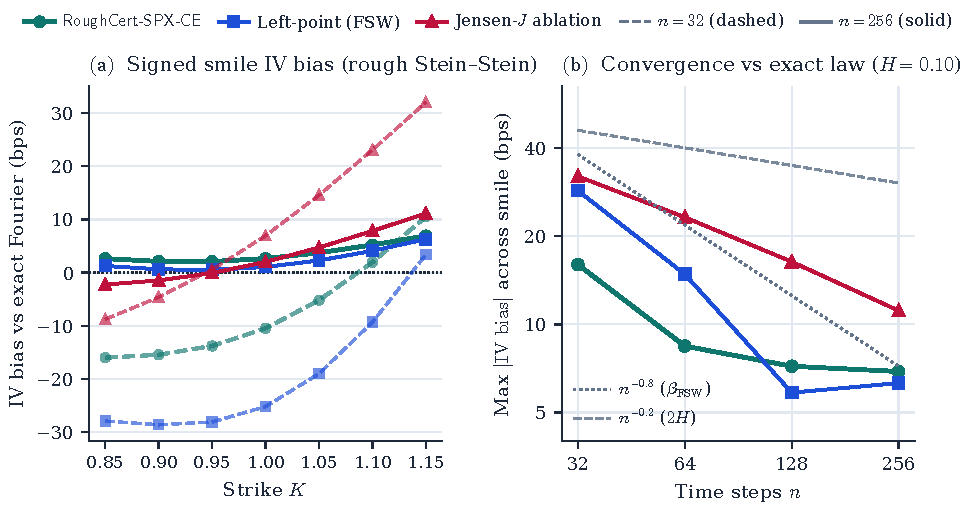
\includegraphics[width=\textwidth]{figures/fig_e1_exact_rss.pdf}
  \caption{Exact-law validation on correlated rough Stein--Stein ($H=0.10$, $T=0.5$, $\rho=-0.7$). (a) IV bias across strikes at $n=32$ and $n=256$ against the $M=\EOneRSSMop$ Fourier reference. (b) Maximum smile IV bias across dyadic levels for \RCCE{}, left-point and the Jensen-$J$ ablation, with reference slopes.}
  \label{fig:e1_rss}
\end{figure}

Three observations follow.
\begin{itemize}
  \item \emph{Containment.} All three envelopes contain the reference price at all seven strikes; the \RCCE{} and left-point envelopes carry \EOneRSSCeDiag{} diagnostic flags. This is consistent with Theorem~\ref{thm:bridge_envelope} on a rough correlated benchmark whose reference has no Monte Carlo error.
  \item \emph{Variance-channel projection reduces coarse-grid error.} At $n=32$, \RCCE{} lowers the maximum smile IV bias from $\EOneRSSLPMaxLow\bps$ (left-point) to $\EOneRSSCeMaxLow\bps$, a reduction by a factor of at least $\EOneRSSCeGainLow$, and the two estimators agree at $n=256$ ($\EOneRSSCeMaxFine\bps$ and $\EOneRSSLPMaxFine\bps$).
  \item \emph{Jensen-$J$ smoothing is worse at every level.} The ablation has the largest bias on every grid ($\EOneRSSJenMaxLow\bps$ at $n=32$ and $\EOneRSSJenMaxFine\bps$ at $n=256$, at least $\EOneRSSJenOverLPFine$ times the left-point value) and $\EOneRSSJenDiag$ diagnostic flags, consistent with the correlation attenuation of Proposition~\ref{prop:jensen_pitfall}(ii).
\end{itemize}

\subsection{Experiment E2: testing the full-determinism hypothesis}
\label{sec:e2}

We compute \emph{Arb-certified} \RCDet{} ATM brackets on a $\ETwoGridNH\times\ETwoGridNEta$ grid of $H\in\{0.05,\allowbreak 0.07,\allowbreak 0.10,\allowbreak 0.15,\allowbreak 0.20,\allowbreak 0.30,\allowbreak 0.40,\allowbreak 0.45\}$ and dimensionless vol-of-vol $\eta_{\mathrm{eff}}=\eta T^H\in[0.02,1.50]$ ($T=0.25$, $\xi_0=0.04$), and locate the $10\bps$, $25\bps$ and $50\bps$ boundaries by $\ETwoBisectSteps$-step bisection (resolution $\ETwoBisectTol$; each boundary is the last certified point) for $\rho=0$ (two-moment bound, Proposition~\ref{prop:twomoment}), $\rho=-0.5$ and $\rho=-0.9$ (Theorem~\ref{thm:put_lipschitz}). Figure~\ref{fig:e2_phase} shows the certifiability landscape, and Table~\ref{tab:e2_spotlights} pairs \RCDet{} with \RCBridge{} in seven spotlight regimes S1--S7.

\begin{figure}[t]
  \centering
  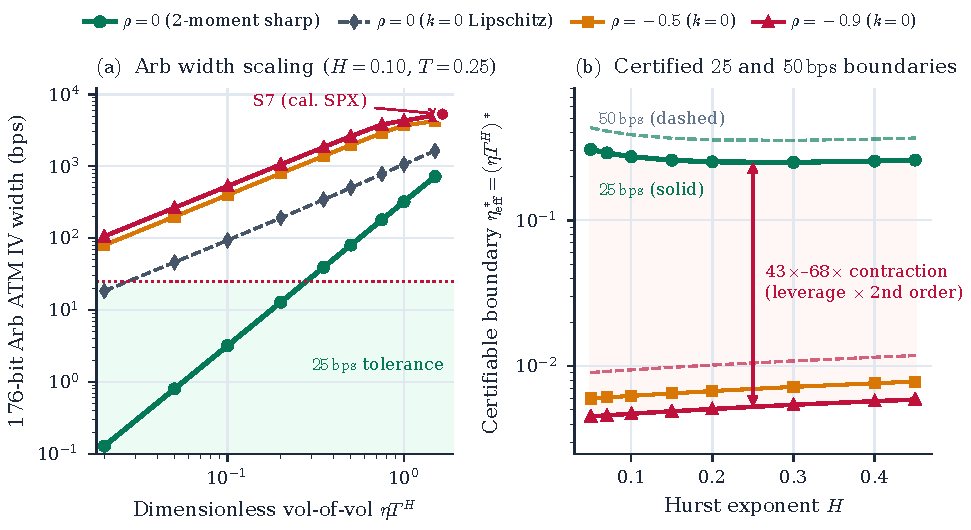
\includegraphics[width=\textwidth]{figures/fig_e2_phase_map.pdf}
  \caption{Deterministic certifiability phase map (ATM, $T=0.25$, $\xi_0=0.04$). (a) Certified IV width against $\eta T^H$ for $\rho=0$ (Proposition~\ref{prop:twomoment}), $\rho=-0.5$ and $\rho=-0.9$ (Theorem~\ref{thm:put_lipschitz}). (b) Certified $25\bps$ and $50\bps$ boundaries across $H$.}
  \label{fig:e2_phase}
\end{figure}

\begin{table}[t]
\centering
\caption{Spotlight comparison of \ArbBits-bit Arb \RCDet{} and \RCBridge{} ATM implied-volatility widths ($\xi_0=0.04$, $25\bps$ desk gate).}
\label{tab:e2_spotlights}
\footnotesize
\setlength{\tabcolsep}{3.6pt}
\begin{tabular}{@{}lrrrrrrlll@{}}
\toprule
Spotlight & $H$ & $T$ & $\eta$ & $\rho$ & Det width & Bridge width & Bridge & Arb & Gate \\
regime & & (yr) & & & (bps, Arb) & (bps, stat.) & status & cont.? & choice \\
\midrule
S1: Mild, $\rho=0$ & 0.30 & 0.10 & 0.30 & $0.0$ & 8.72 & 0.02 & Asymp.-env. & Yes & Tier~1 (Arb) \\
S2: Rough, $\rho=0$ & 0.10 & 0.25 & 0.20 & $0.0$ & 9.21 & 0.03 & Asymp.-env. & Yes & Tier~1 (Arb) \\
S3: 1-day, corr. & 0.30 & $1/252$ & 0.03 & $-0.7$ & 22.54 & 0.12 & Asymp.-env. & Yes & Tier~1 (Arb) \\
S4: Rough, mild $\eta$ & 0.10 & 0.25 & 0.10 & $-0.7$ & 413.0 & 0.44 & Asymp.-env. & Yes & Tier~3 (Bridge) \\
S5: Rough, mod.\ $\eta$ & 0.10 & 0.25 & 0.50 & $-0.7$ & 2044.3 & 5.59 & Asymp.-env. & Yes & Tier~3 (Bridge) \\
S6: Cal.\ $\eta$, $\rho=0$ & 0.10 & 0.25 & 1.90 & $0.0$ & 823.3 & 9.64 & Asymp.-env. & Yes & Tier~3 (Bridge) \\
S7: Cal.\ SPX full & 0.10 & 0.25 & 1.90 & $-0.9$ & 5301.8 & 18.43 & Asymp.-env. & Yes & Tier~3 (Bridge) \\
\bottomrule
\end{tabular}
\par\smallskip
\parbox{\linewidth}{\footnotesize\emph{Notes.} Det: deterministic Arb-certified ATM IV width (Proposition~\ref{prop:twomoment} for $\rho=0$, Theorem~\ref{thm:put_lipschitz} for $\rho<0$). Bridge: asymptotic-envelope statistical(0.95) width (Theorem~\ref{thm:bridge_envelope}; levels $32$--$256$, $32{,}768$ RQMC paths). The two widths carry different guarantees. Arb cont.: the Arb bracket contains the Bridge midpoint.}
\end{table}
%

Experiment~E2 settles the hypothesis quantitatively.
\begin{enumerate}[1.]
  \item \emph{Zero leverage.} The two-moment bound is of second order and certifies ATM IV to $25\bps$ up to $\eta T^H\in[\ETwoRhoZeroMin,\ETwoRhoZeroMax]$ across $H\in[0.05,0.45]$, which is $\ETwoSecondOrderMin$--$\ETwoSecondOrderMax$ times further than the first-order bracket reaches at $\rho=0$ ($\eta T^H\in[\ETwoRhoZeroFirstMin,\ETwoRhoZeroFirstMax]$). Spotlights S1 ($\ETwoSOneDet\bps$) and S2 ($\ETwoSTwoDet\bps$, $H=0.10$) pass the desk gate in Arb alone.
  \item \emph{Leverage.} At $\rho=-0.9$ the $25\bps$ boundary drops to $\eta T^H\in[\ETwoRhoNineMin,\ETwoRhoNineMax]$, a contraction by a factor of $\ETwoCollapseMin$--$\ETwoCollapseMax$. It factors into a leverage factor of $\ETwoLeverageMin$--$\ETwoLeverageMax$, obtained with the same first-order bracket at $\rho=0$ and $\rho=-0.9$, and the second-order factor above, which is lost because the two-moment bound exists only at $\rho=0$ (Supplementary Table~S2). The leverage factor is almost constant in $H$ because both first-order brackets scale with the same residual $E_J$; they differ through the coefficients of Theorem~\ref{thm:put_lipschitz} and through the concavity cap $C(1)\le C_\BS(1,1,\E[I_T])$ that tightens the $\rho=0$ bracket from above. Only very short or very mild regimes such as S3 (one-day maturity, $\ETwoSThreeDet\bps$) pass deterministically.
  \item \emph{Calibrated SPX parameters need Tier~3.} At S7 ($H=0.10$, $T=0.25$, $\eta=1.9$, $\rho=-0.9$), \RCDet{} gives a deterministic envelope of width $\ETwoSSevenDet\bps$, which contains the Bridge midpoint as in all seven spotlights. The \RCBridge{} envelope is $\ETwoSSevenBridge\bps$ wide, narrower by a factor of at least $\ETwoSSevenRatio$, but it carries the \emph{asymptotic-envelope statistical(0.95)} label rather than a deterministic guarantee; all seven spotlights reach that status, with widths down to $\ETwoSFourBridge\bps$ at S4.
\end{enumerate}
A code-disjoint recomputation with the exact formulas (checks I1--I2, Supplementary Table~S5) confirms that every stored Arb bracket contains the exact-formula bracket and that the exact ATM width at the stored $25\bps$ boundary points for $H=0.10$ and $H=0.30$ is at most $\IndepETwoMaxExactWidth\bps$. The Arb brackets are wider than the exact-formula brackets by $\ETwoArbOverheadMin$--$\ETwoArbOverheadMax\%$, mostly in the $\rho=0$ spotlights, where the box enclosure of $\Var(I_T)$ enters the two-moment bound.

\FloatBarrier
%
\section{Kernel audits, head-to-head benchmarks and weak rates}
\label{sec:benchmarks}

We now address three questions faced by volatility desks and model validators: (i) how large the continuous-time kernel-approximation error of Markovian and hybrid schemes can be, certified in Arb (Experiment~E3); (ii) how six published SPX pricing families compare against a continuum enclosure in three market regimes (Experiment~E4); and (iii) how measured weak rates compare with $\beta_{\mathrm{FSW}}(H)$ and with the Jensen-$J$ ablation of Proposition~\ref{prop:jensen_pitfall} (Experiment~E5).

\subsection{Experiment E3: continuous-time kernel audit in Arb}
\label{sec:e3}

Before any Markovian or hybrid simulation, Theorem~\ref{thm:put_lipschitz} bounds the continuous-time kernel gap $|C(K)-C_{\hat{K}}(K)|$ in Arb. We audit \citet{BayerBreneis2023} exponential sums fitted by unclipped, preconditioned L-BFGS-B ($M\in\{2,4,6,8,12,16\}$ factors, $H\in\{0.07,0.10,0.30\}$) and \citet{BennedsenLundePakkanen2017} hybrid kernels ($\kappa\in\{1,2,3,4,6,8\}$, $n=256$) on calibrated rough Bergomi ($T=0.25$, $\eta=1.9$, $\rho=-0.9$, $\xi_0=0.04$). At $H=0.10$ the empirical errors are measured against a $131{,}072$-path \RCBridge{} reference on levels $(64,128,256,512)$ with ATM implied volatility $[\EThreeRefATMLo,\EThreeRefATMHi]\%$ (width $\EThreeRefATMW\bps$) and finite-difference ATM skew $[\EThreeRefSkewLo,\EThreeRefSkewHi]$ ($\delta k=0.02$). Table~\ref{tab:e3_kernel} and Figure~\ref{fig:e3_kernel} summarise the results.

\begin{table}[t]
\centering
\caption{\ArbBits-bit Arb continuous-time kernel audit at $H=0.10$, $T=0.25$, $\eta=1.9$, $\rho=-0.9$, $\xi_0=0.04$.}
\label{tab:e3_kernel}
\footnotesize
\setlength{\tabcolsep}{4.0pt}
\begin{tabular}{@{}lrrrrrrr@{}}
\toprule
Kernel approximation & $\|K{-}\hat{K}\|_{L^2}$ & $\|K{-}\hat{K}\|_{L^1}$ & $E_J$ upper & Price gap & Fit & ATM IV err & Emp.\ ATM \\
 & (Arb) & (Arb) & (Arb) & (Arb) & (s) & (bps, stat.) & skew \\
\midrule
BB2023 ($M=2$) & 0.3254 & 0.05556 & 0.02989 & 0.03452 & 0.13 & $[12.6,\,21.5]$ & $-0.6117$ \\
BB2023 ($M=4$) & 0.1747 & 0.02805 & 0.01622 & 0.01873 & 0.19 & $[0.0,\,5.8]$ & $-0.5985$ \\
BB2023 ($M=6$) & 0.1044 & 0.01584 & 0.00973 & 0.01124 & 0.35 & $[0.0,\,7.2]$ & $-0.5932$ \\
BB2023 ($M=8$) & 0.0665 & 0.00957 & 0.00621 & 0.00717 & 0.51 & $[0.0,\,8.6]$ & $-0.5919$ \\
BB2023 ($M=12$) & 0.0304 & 0.00402 & 0.00285 & 0.00329 & 1.03 & $[0.0,\,5.1]$ & $-0.5944$ \\
BB2023 ($M=16$) & 0.0155 & 0.00192 & 0.00145 & 0.00168 & 2.80 & $[0.0,\,4.6]$ & $-0.5948$ \\
\midrule
BLP hybrid ($\kappa=1$, $n=256$) & -- & -- & 0.00175 & 0.00202 & -- & $\le 101.0^{\ddagger}$ & -- \\
BLP hybrid ($\kappa=2$, $n=256$) & -- & -- & 0.00096 & 0.00111 & -- & $\le 55.6^{\ddagger}$ & -- \\
BLP hybrid ($\kappa=4$, $n=256$) & -- & -- & 0.00052 & 0.00060 & -- & $\le 29.9^{\ddagger}$ & -- \\
BLP hybrid ($\kappa=8$, $n=256$) & -- & -- & 0.00028 & 0.00032 & -- & $\le 15.8^{\ddagger}$ & -- \\
\bottomrule
\end{tabular}
\par\smallskip
\parbox{\linewidth}{\footnotesize\emph{Notes.} Upper panel: unclipped L-BFGS-B factors of \citet{BayerBreneis2023}; columns 2--5 are Arb-certified upper bounds; the ATM error interval ($n=256$) is statistical, against the \RCBridge{} reference ATM IV $[\EThreeRefATMLo,\EThreeRefATMHi]\%$. Lower panel: continuous-time hybrid kernel. $^{\ddagger}$Certified gap mapped to IV across the statistical reference bracket (conditional; time stepping excluded).}
\end{table}
%

\begin{figure}[t]
  \centering
  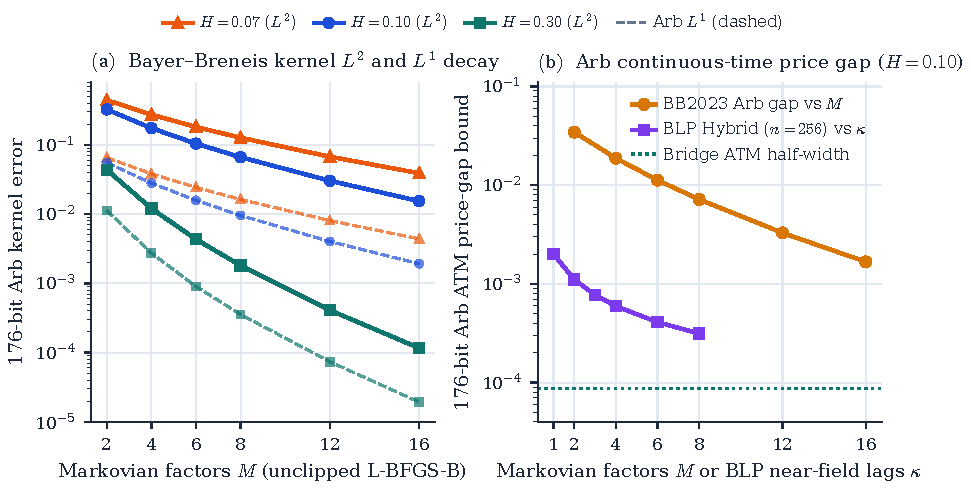
\includegraphics[width=\textwidth]{figures/fig_e3_kernel_audit.pdf}
  \caption{Continuous-time kernel audit in Arb ($T=0.25$, $\eta=1.9$, $\rho=-0.9$, $\xi_0=0.04$). (a) Certified $L^2$ (solid) and root-splitting $L^1$ (dashed) errors of unclipped \citet{BayerBreneis2023} kernels for $H\in\{0.07,0.10,0.30\}$. (b) Certified ATM price-gap bounds for Markovian factors $M$ and hybrid lags $\kappa$ at $H=0.10$.}
  \label{fig:e3_kernel}
\end{figure}

Three findings bear on kernel selection.
\begin{enumerate}[1.]
  \item \emph{Geometric decay of the Markovian kernel error.} Without artificial upper bounds on the mean-reversion speeds $x_j$, which stall the decay at small $H$, the certified $L^2$ error at $H=0.10$ falls from $\EThreeMkTenMTwoLTwo$ ($M=2$) to $\EThreeMkTenMSixteenLTwo$ ($M=16$, fit time $\EThreeMkTenMSixteenFit\,\mathrm{s}$), and the certified $L^1$ error reaches $\EThreeMkTenMSixteenLOne$. With $M=16$ the certified $L^2$ error is $\EThreeMkSevenMSixteenLTwo$ at $H=0.07$ and $\EThreeMkThirtyMSixteenLTwo$ at $H=0.30$.
  \item \emph{The price-gap certificate is conservative at calibrated vol-of-vol.} At $H=0.10$ and $M=16$, Theorem~\ref{thm:put_lipschitz} bounds the continuous-time ATM price gap by $\EThreeMkTenMSixteenGap$, about $\EThreeMkTenMSixteenGapIV\bps$ in implied volatility, whereas the empirical ATM IV error against \RCBridge{} is at most $\EThreeMkTenMSixteenATMHi\bps$, smaller by a factor of at least $\EThreeMkGapOverEmp$. The bound is first order in $E_J$ and admits no cancellation; its value lies in holding before any simulation and in decaying geometrically with $M$ (about $\EThreeMkTenMTwelveGapIV\bps$ at $M=12$). The empirical ATM error interval itself contracts from at least $\EThreeMkTenMTwoATMLo\bps$ ($M=2$) to at most $\EThreeMkTenMSixteenATMHi\bps$ ($M=16$).
  \item \emph{Hybrid kernel gap.} Propagating the certified continuous-time hybrid price gap across the statistical reference ATM price bracket bounds the IV gap by $\EThreeBLPKapOneIV\bps$ ($\kappa=1$), $\EThreeBLPKapTwoIV\bps$ ($\kappa=2$), $\EThreeBLPKapFourIV\bps$ ($\kappa=4$) and $\EThreeBLPKapEightIV\bps$ ($\kappa=8$) at $n=256$. These IV figures inherit the statistical status of the reference bracket, and they exclude discrete time-stepping error by construction. A code-disjoint evaluation of $E_J$ for the hybrid kernels lies inside every stored Arb ball (check~I3).
\end{enumerate}

\subsection{Experiment E4: head-to-head SPX benchmarks in three regimes}
\label{sec:e4}

We benchmark six published SPX rough-Bergomi pricing families on identical single-threaded hardware, reporting \emph{cold setup time} and \emph{amortised solve time} separately, with error intervals $[\operatorname{dist}(v,[L,U]),\max(|v-L|,|v-U|)]$ against a $131{,}072$-path \RCBridge{} reference on levels $(64,128,256,512)$:
\begin{itemize}
  \item \emph{Regime~A (calibrated three-month SPX):} $H=0.10$, $T=0.25$, $\eta=1.9$, $\rho=-0.9$, $\xi_0=0.04$, eight strikes in $[0.85,1.12]$ including the skew stencil $e^{\pm 0.02}$; reference ATM IV $[\EFourARefATMLo,\EFourARefATMHi]\%$ (width $\EFourARefATMW\bps$, $\EFourARefDiag$ diagnostic strike at $K=0.85$) and ATM skew $[\EFourARefSkewLo,\EFourARefSkewHi]$.
  \item \emph{Regime~B (ultra-rough one-month SPX):} $H=0.07$, $T=1/12$, $\eta=1.9$, $\rho=-0.9$, $\xi_0=0.235^2$, seven strikes in $[0.90,1.08]$ including $e^{\pm 0.015}$; reference ATM IV $[\EFourBRefATMLo,\EFourBRefATMHi]\%$ (width $\EFourBRefATMW\bps$, $\EFourBRefDiag$ diagnostic strikes at $K\in\{0.95,1.05\}$) and ATM skew $[\EFourBRefSkewLo,\EFourBRefSkewHi]$.
  \item \emph{Regime~C (curved forward variance, six months):} $H=0.10$, $T=0.50$, $\eta=1.9$, $\rho=-0.85$, $\xi_0(t)=0.234^2(1+t)^2$, seven strikes in $[0.80,1.20]$ including $e^{\pm 0.02}$; reference ATM IV $[\EFourCRefATMLo,\EFourCRefATMHi]\%$ (width $\EFourCRefATMW\bps$, no diagnostic strike) and ATM skew $[\EFourCRefSkewLo,\EFourCRefSkewHi]$.
\end{itemize}
Every simulated competitor uses the same main budget of $32{,}768$ paths ($R=16$ shifts of $2{,}048$ antithetic paths) and a sampling-type label. Scrambled Sobol RQMC with the pilot-fitted control bank ($R_{\mathrm{pilot}}=2$ extra pilot shifts, timed inside the solve time) is used for \RCCE{} and for the Brownian-bridge left-point RQMC of \citet{BayerBenHammoudaTempone2020}, whose Richardson extrapolation is labelled \emph{diagnostic}. Pseudo-random antithetic MC with Romano--Touzi conditioning and two-control leave-one-shift-out cross-fitting is used for the hybrid scheme of \citet{McCrickerdPakkanen2018} ($\kappa\in\{1,2\}$), the Markovian scheme of \citet{BayerBreneis2023} and the rDonsker scheme of \citet{HorvathJacquierMuguruza2024}, whose Eq.~(4.2) gives the variance-matched (vm) cell weight $(\Delta t^{-1}\int_{\rm cell}K_H^2)^{1/2}$. Our comparison also uses the cell mean $\Delta t^{-1}\int_{\rm cell}K_H$, the $L^2$ projection evaluated at the optimal point $b_k^*$ of \citet{BennedsenLundePakkanen2017}. The order-two expansion of \citet{BergomiGuyon2012} is analytic and labelled \emph{diagnostic}. In tables and figures these competitors appear as BHT2020, MP2018, BB2023, HJMS2024 and BG2012. The simulated methods share common random numbers, which sharpens comparisons without affecting the validity of each marginal interval (\ref{app:repro}). Tables~\ref{tab:e4_regimeA}--\ref{tab:e4_regimesBC} and Figures~\ref{fig:e4_dot}--\ref{fig:e4_wp} report the results.

\begin{table}[t]
\centering
\caption{Head-to-head SPX benchmarks in Regime~A ($H=0.10$, $T=0.25$, $\eta=1.9$, $\rho=-0.9$, $\xi_0=0.04$, $8$ strikes in $[0.85,1.12]$).}
\label{tab:e4_regimeA}
\footnotesize
\setlength{\tabcolsep}{3.6pt}
\begin{tabular}{@{}llrrrrrr@{}}
\toprule
Method & Type & Setup & Solve & ATM IV err & Max smile err & ATM & Skew err \\
($32{,}768$ paths; 1 thread) & & (s) & (s) & (bps) & (bps) & skew & interval \\
\midrule
\RCCE{} ($n=128$) & RQMC & 0.06 & 2.27 & $[0.0,\,7.7]$ & $[0.0,\,67.8]$ & $-0.590$ & $[0.000,\,0.056]$ \\
\RCCE{} ($n=256$) & RQMC & 0.38 & 4.80 & $[0.0,\,7.8]$ & $[0.0,\,55.5]$ & $-0.594$ & $[0.000,\,0.052]$ \\
Jensen-$J$ ablation ($n=256$) & RQMC & 0.38 & 9.48 & $[3.9,\,17.4]$ & $[3.9,\,57.9]$ & $-0.590$ & $[0.000,\,0.056]$ \\
BHT2020 Bridge-RQMC ($n=128$) & RQMC & 0.01 & 1.87 & $[0.0,\,7.2]$ & $[2.1,\,83.6]$ & $-0.589$ & $[0.000,\,0.057]$ \\
BHT2020 Bridge-RQMC ($n=256$) & RQMC & 0.06 & 3.59 & $[0.0,\,8.8]$ & $[0.0,\,61.9]$ & $-0.590$ & $[0.000,\,0.056]$ \\
BHT2020 Richardson (64,128) & Diag. & 0.01 & 2.87 & $[0.0,\,8.2]$ & $[0.9,\,66.9]$ & $-0.608$ & $[0.000,\,0.059]$ \\
MP2018 hybrid ($\kappa=1,n=128$) & MC & 0.00 & 0.88 & $[0.0,\,7.0]$ & $[2.6,\,82.5]$ & $-0.585$ & $[0.000,\,0.061]$ \\
MP2018 hybrid ($\kappa=2,n=256$) & MC & 0.01 & 2.26 & $[0.0,\,6.9]$ & $[0.0,\,61.6]$ & $-0.594$ & $[0.000,\,0.051]$ \\
BB2023 Markov ($M=8,n=128$) & MC & 0.57 & 2.15 & $[0.0,\,7.4]$ & $[0.8,\,80.7]$ & $-0.588$ & $[0.000,\,0.058]$ \\
BB2023 Markov ($M=12,n=256$) & MC & 1.10 & 5.32 & $[0.0,\,13.2]$ & $[0.0,\,67.8]$ & $-0.587$ & $[0.000,\,0.059]$ \\
HJMS2024 rDonsker (vm, $n=256$) & MC & 0.00 & 1.74 & $[5.5,\,19.1]$ & $[7.6,\,59.8]$ & $-0.614$ & $[0.000,\,0.065]$ \\
rDonsker (BLP $b_k^*$, $n=256$) & MC & 0.00 & 1.76 & $[2.0,\,15.6]$ & $[34.2,\,115.7]$ & $-0.624$ & $[0.000,\,0.074]$ \\
BG2012 order-2 expansion & Diag. & 0.00 & 0.00 & $[42.9,\,56.5]$ & $[295.4,\,376.9]$ & $-0.681$ & $[0.036,\,0.132]$ \\
\bottomrule
\end{tabular}
\par\smallskip
\parbox{\linewidth}{\footnotesize\emph{Notes.} Errors: $[\operatorname{dist}(v,[L,U]),\max(|v-L|,|v-U|)]$ for the point estimate $v$ against the $131{,}072$-path \RCBridge{} reference (ATM IV $[\EFourARefATMLo,\EFourARefATMHi]\%$, skew $[\EFourARefSkewLo,\EFourARefSkewHi]$); the sampling error of $v$ is not included. Type: scrambled-Sobol RQMC, pseudo-random MC, analytic or diagnostic. Simulated methods share common random numbers.}
\end{table}
%

\begin{figure}[t]
  \centering
  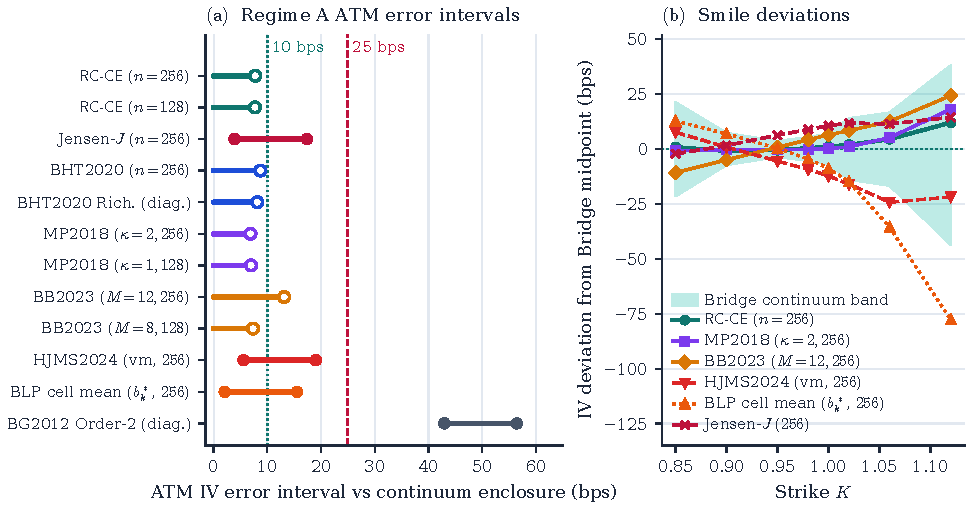
\includegraphics[width=\textwidth]{figures/fig_e4_dot_table.pdf}
  \caption{Head-to-head SPX benchmarks in Regime~A ($H=0.10$, $T=0.25$, $\eta=1.9$, $\rho=-0.9$). (a) ATM IV error intervals against the $131{,}072$-path \RCBridge{} enclosure; open circles mark zero lower distance. (b) Signed smile deviations from the Bridge midpoint across $K\in[0.85,1.12]$.}
  \label{fig:e4_dot}
\end{figure}

\begin{figure}[t]
  \centering
  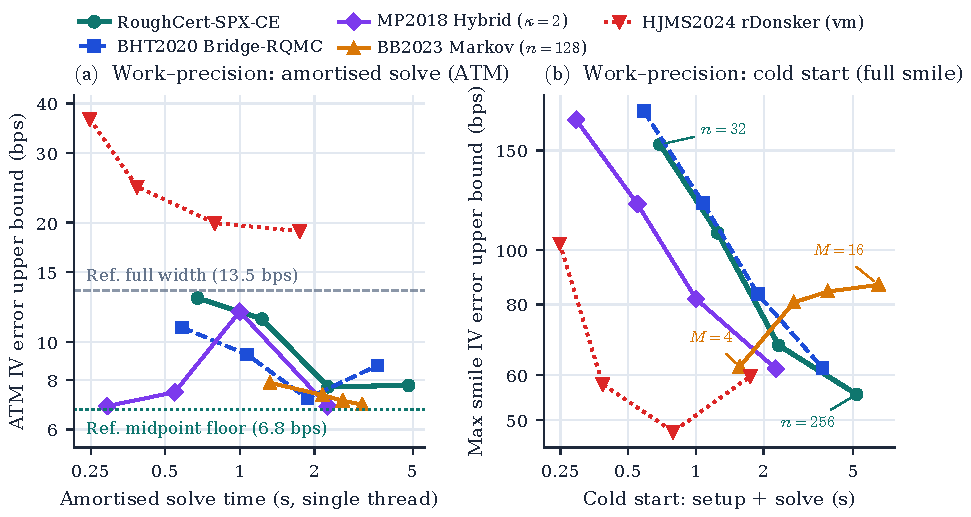
\includegraphics[width=\textwidth]{figures/fig_e4_work_precision.pdf}
  \caption{Work--precision curves in Regime~A ($32{,}768$ paths, one thread). (a) Upper end of the ATM IV error against amortised solve time, with the reference midpoint floor $W/2$. (b) Upper end of the maximum smile IV error over $K\in[0.85,1.12]$ against cold-start time (setup plus solve).}
  \label{fig:e4_wp}
\end{figure}

\begin{table}[t]
\centering
\caption{Head-to-head benchmarks in Regime~B (ultra-rough one-month, $H=0.07$) and Regime~C (curved $\xi_0(t)$, $T=0.50$).}
\label{tab:e4_regimesBC}
\footnotesize
\begin{tabular}{@{}llrrrr@{}}
\toprule
Regime and method & Type & Solve (s) & ATM IV err (bps) & Max smile err (bps) & ATM skew \\
\midrule
B: \RCCE{} ($n=128$) & RQMC & 2.32 & $[0.0,\,7.6]$ & $[0.0,\,91.3]$ & $-0.865$ \\
B: BHT2020 ($n=128$) & RQMC & 2.48 & $[0.0,\,9.4]$ & $[1.7,\,91.9]$ & $-0.866$ \\
B: MP2018 ($\kappa=2,n=128$) & MC & 1.38 & $[0.0,\,8.4]$ & $[2.4,\,95.2]$ & $-0.863$ \\
B: BB2023 ($M=12,n=128$) & MC & 3.10 & $[0.0,\,9.2]$ & $[0.8,\,89.3]$ & $-0.874$ \\
B: HJMS2024 (vm, $n=128$) & MC & 0.79 & $[13.4,\,27.4]$ & $[19.1,\,121.3]$ & $-0.944$ \\
B: BG2012 order-2 & Diag. & 0.00 & $[34.0,\,48.1]$ & $[276.1,\,358.2]$ & $-1.030$ \\
\midrule
C: \RCCE{} ($n=128$) & RQMC & 3.07 & $[0.0,\,9.4]$ & $[0.0,\,51.4]$ & $-0.426$ \\
C: BHT2020 ($n=128$) & RQMC & 2.54 & $[0.0,\,8.0]$ & $[0.0,\,67.1]$ & $-0.423$ \\
C: MP2018 ($\kappa=2,n=128$) & MC & 1.42 & $[0.0,\,8.2]$ & $[5.0,\,76.0]$ & $-0.421$ \\
\bottomrule
\end{tabular}
\par\smallskip
\parbox{\linewidth}{\footnotesize\emph{Notes.} Regime~B ($H=0.07$, $T=1/12$, $\eta=1.9$, $\rho=-0.9$, $\xi_0=0.235^2$): \RCBridge{} ATM IV $[\EFourBRefATMLo,\EFourBRefATMHi]\%$, skew $[\EFourBRefSkewLo,\EFourBRefSkewHi]$. Regime~C ($H=0.10$, $T=0.50$, $\eta=1.9$, $\rho=-0.85$, $\xi_0(t)=0.234^2(1+t)^2$): ATM IV $[\EFourCRefATMLo,\EFourCRefATMHi]\%$, skew $[\EFourCRefSkewLo,\EFourCRefSkewHi]$. Error intervals as in Table~\ref{tab:e4_regimeA}.}
\end{table}
%

Five lessons emerge across Regimes~A--C.
\begin{enumerate}[1.]
  \item \emph{Exact-grid \RCCE{} and BHT2020 track the reference closely.} In Regime~A, the ATM IV error of \RCCE{} is at most $\EFourACEOneTwoEightATMHi\bps$ at $n=128$ and $\EFourACETwoFiveSixATMHi\bps$ at $n=256$ (solve time $\EFourACETwoFiveSixSolve\,\mathrm{s}$), with zero lower distance across the smile core. The Jensen-$J$ ablation at $n=256$ behaves differently: its 95\% confidence interval at the money lies $\EFourAJenTwoFiveSixATMCIDist\bps$ above the reference envelope, and its point estimate is at least $\EFourAJenTwoFiveSixMaxLo\bps$ from the envelope somewhere on the smile, consistent with Proposition~\ref{prop:jensen_pitfall}.
  \item \emph{The MP2018 hybrid scheme ($\kappa=2$) is fastest after amortisation, but its bias needs an external audit.} It solves in $\EFourAMPTwoTwoFiveSixSolve\,\mathrm{s}$ at $n=256$ ($\EFourAMPTwoOneTwoEightSolve\,\mathrm{s}$ at $n=128$) with ATM error at most $\EFourAMPTwoTwoFiveSixATMHi\bps$. A single-grid run does not bound its own time-step bias; that requires an \RCBridge{} or Arb kernel audit.
  \item \emph{The unclipped BB2023 Markovian scheme ($M=12$) is accurate once its setup is amortised.} After the $\EFourABBMTwelveSetup\,\mathrm{s}$ one-time kernel fit, it solves in $\EFourABBMTwelveSolveTwoFiveSix\,\mathrm{s}$ at $n=256$ with zero lower distance across the smile. At $n=128$ (Figure~\ref{fig:e4_wp}(b)), increasing $M$ from $4$ to $16$ slightly raises the upper smile error, which we attribute to the fixed-$n$ Euler bias that remains once the kernel truncation is removed.
  \item \emph{The rDonsker weight choice matters.} With variance-matched weights (terminal variance ratio $\EFourARDVmVarRatio$), the maximum smile error is at most $\EFourARDVmTwoFiveSixMaxHi\bps$ at $n=256$. The optimal weights $b_k^*$ give a terminal variance ratio of $\EFourARDBsVarRatio$ at $n=256$ (a deficit of $\EFourARDBsDeficitPct\%$; $\EFourARDBsVarRatioSixtyFour$ at $n=64$) and a maximum smile error of at least $\EFourARDBsTwoFiveSixMaxLo\bps$. At the money alone, the variance deficit partly cancels the left-point Euler bias, so ATM spot checks can mislead and full-smile audits are needed.
  \item \emph{BG2012 fails at calibrated vol-of-vol.} The order-two expansion reproduces its $O(\eta^3)$ and $O(\eta^4)$ error orders for small $\eta$ (unit test~5 of the code archive), but at $\eta=1.9$ its maximum smile error exceeds $\EFourABGMaxLo\bps$ in Regime~A and $\EFourBBGMaxLo\bps$ in Regime~B, with ATM skew error above $\EFourBBGSkewLo$; it stays \emph{diagnostic}. In Regimes~B and~C, \RCCE{} stays inside or close to the reference under $H=0.07$ and under the curved forward variance; in Regime~B the two diagnostic reference strikes govern the upper smile errors in Table~\ref{tab:e4_regimesBC}.
\end{enumerate}

\paragraph{Refinement of the diagnostic reference strikes.}
The diagnostic strikes of the Regime~A and~B references (and of two E6 rows, Section~\ref{sec:joint}) were recomputed with one more dyadic level ($n_L=\RefFinestLevel$), the same path budgets and fresh seeds (Supplementary Table~S1). In Regime~A the deep put $K=0.85$ reaches asymptotic-envelope status and its width shrinks from $\RefAWidthLowKVOne\bps$ to $\RefAWidthLowKVTwo\bps$; in Regime~B both wing strikes are upgraded ($\RefBWidthNineFiveVOne\to\RefBWidthNineFiveVTwo\bps$ at $K=0.95$ and $\RefBWidthOneOFiveVOne\to\RefBWidthOneOFiveVTwo\bps$ at $K=1.05$). The conclusions of this subsection are unchanged against the refined references: the BG2012 lower error stays above $\IndepBGMinLoRefined\bps$, and the Jensen-$J$ lower smile error at $n=256$ becomes $\IndepJenMaxLoRefined\bps$ (check~I7).

\subsection{Experiment E5: weak rates across the FSW phase transition}
\label{sec:e5}

Experiment~E5 measures coupled dyadic increments on six grids from $n=16$ to $n=512$, with $65{,}536$ scrambled Sobol paths and the control bank, for five Hurst indices $H\in\{0.05,\allowbreak 0.10,\allowbreak 0.15,\allowbreak 0.25,\allowbreak 0.40\}$ at $T=0.25$, $\eta=1.9$, $\rho=-0.9$, $\xi_0=0.04$ and $K\in\{0.95,1.00,1.06\}$, and compares the fitted log--log rates $\hat{\beta}$ with $\beta_{\mathrm{FSW}}(H)$. The call wing $K=1.06$ has monotone same-sign increments with high signal-to-noise ratio for all five $H$; Figure~\ref{fig:e5_rates}(a) plots its rates against $\beta_{\mathrm{FSW}}(H)$ and the line $2H$, and Figure~\ref{fig:e5_rates}(b) shows the increment magnitudes $|\bar{\Delta}_n|$ at $H=0.10$.

\begin{figure}[t]
  \centering
  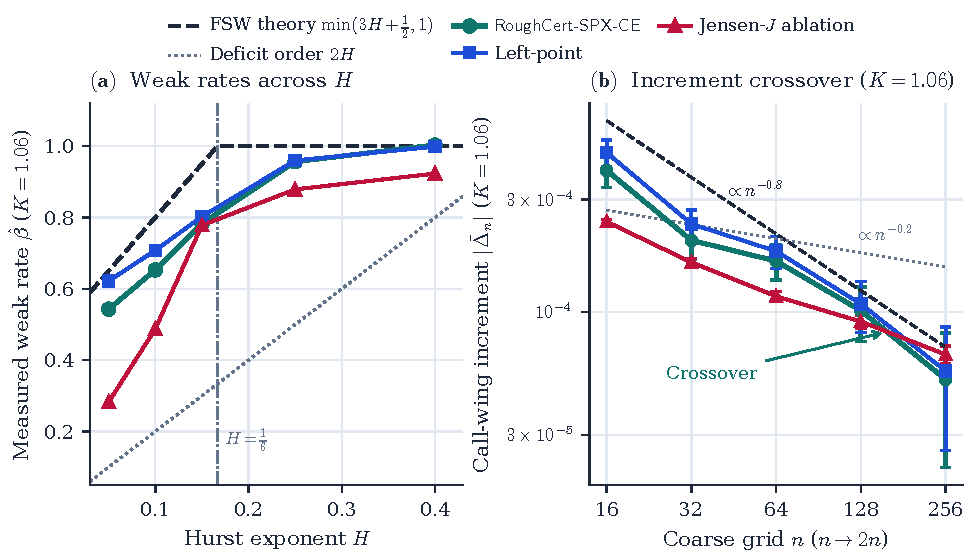
\includegraphics[width=\textwidth]{figures/fig_e5_weak_rates.pdf}
  \caption{Measured weak rates across $H\in[0.05,0.40]$ ($65{,}536$ paths, $n\in[16,512]$, $\eta=1.9$, $\rho=-0.9$). (a) Rate $\hat{\beta}$ at $K=1.06$ against $\min(3H+\tfrac12,1)$ \citep{FrizSalkeldWagenhofer2025} and the line $2H$. (b) Coupled increment magnitudes at $H=0.10$ with 95\% bars.}
  \label{fig:e5_rates}
\end{figure}

\begin{itemize}
  \item \emph{The FSW phase transition.} The left-point and \RCCE{} rates rise with $H$ and saturate near one for $H\ge 0.25$, as $\beta_{\mathrm{FSW}}$ predicts. At $K=1.06$ the left-point rates are $\EFiveLPHZeroFive$, $\EFiveLPHTen$, $\EFiveLPHFifteen$, $\EFiveLPHTwoFive$ and $\EFiveLPHForty$ for $H=0.05,0.10,0.15,0.25,0.40$, and the \RCCE{} rates are $\EFiveCEHZeroFive$, $\EFiveCEHTen$, $\EFiveCEHFifteen$, $\EFiveCEHTwoFive$ and $\EFiveCEHForty$. For $H\le0.15$ these single-strike rates lie below $\beta_{\mathrm{FSW}}(H)$, a pre-asymptotic effect on the tested grids, while the \RCCE{} strip-mean rate at $H=0.10$ ($\EFiveTenStripCE$) matches $\beta_{\mathrm{FSW}}(0.10)=0.80$.
  \item \emph{Support for Case~(ii) of Theorem~\ref{thm:bridge_envelope}.} For every tested $H\ge0.10$, all measured left-point and \RCCE{} rates (at $K=1.06$, at the money and on the strip mean) exceed the floor $\beta_{\min}(H)$, with margin at least $\EFiveMinMargin$ (check~C7b). At $H=0.05$ three rates fall below $\beta_{\min}(0.05)=\BetaMinZeroFive$ (\RCCE{} strip mean $\EFiveStripCEHZeroFive$, left-point strip mean $\EFiveStripLPHZeroFive$, \RCCE{} ATM $\EFiveATMCEHZeroFive$), so Case~(ii) envelopes are not supported there. Regime~B ($H=0.07$) lies between the tested values. Of all $\CaseTotalCount$ reference-envelope strikes in E1, E3, E4 and E6, $\CaseOneCount$ are in Case~(i), $\CaseTwoCount$ in Case~(ii) and $\CaseThreeCount$ are diagnostic (Supplementary Table~S3), so Case~(ii) carries most envelopes.
  \item \emph{Slower decay of the Jensen-$J$ ablation.} At $K=1.06$ the ablation's rates are $\EFiveJenHZeroFive$, $\EFiveJenHTen$, $\EFiveJenHFifteen$ and $\EFiveJenHTwoFive$ for $H=0.05,0.10,0.15,0.25$, below the \RCCE{} rates. The gap is negligible at $H=0.15$, where the ablation's ATM rate ($\EFiveATMFifteenJen$ against $\EFiveATMFifteenCE$) and strip-mean rate ($\EFiveStripFifteenJen$ against $\EFiveStripFifteenCE$) remain clearly lower; at $H=0.10$ its strip-mean rate is $\EFiveTenStripJen$ against $\EFiveTenStripCE$. Every resolved ablation rate exceeds $2H$, so the order suggested by the heuristic of Section~\ref{sec:jensen_pitfall} is not observed on these grids. Panel~(b) shows a crossover at $H=0.10$, $K=1.06$: on the coarsest grid the ablation's increment ($\EFiveTenJenCoarse$) is smaller than those of \RCCE{} ($\EFiveTenCECoarse$) and left-point ($\EFiveTenLPCoarse$), but it decays more slowly, and by $n=256$ the \RCCE{} point estimate ($\EFiveTenCEFine$) lies below the ablation's ($\EFiveTenJenFine$), with overlapping 95\% bars. A coarse-grid comparison alone would therefore favour the ablation despite its slower measured convergence.
\end{itemize}

\FloatBarrier
%
\section{Experiment E6: joint SPX--VIX consistency audit}
\label{sec:joint}

Joint calibration of SPX and VIX implied-volatility surfaces is a long-standing difficulty for rough volatility \citep{Guyon2020,Romer2022,BourgeyDeMarcoGobet2023,AbiJaberIllandLi2025}: one-component rough Bergomi models fit steep short-dated SPX smiles but tend to produce nearly flat VIX smiles, whereas the two-component mixed model \eqref{eq:mixed_rbergomi} adds vol-of-vol convexity that lifts the VIX smile. When both legs come from single-grid Monte Carlo, genuine model rigidity is hard to separate from coarse time-stepping bias in the SPX skew.

Experiment~E6 places the 169-bit \emph{Arb-certified} VIX futures and VIX smile brackets of the companion working paper and software release \RoughCert{} \CompanionTag{} \citep{AhmedEtAl2026RoughCert} beside $65{,}536$-path \RCBridge{} (\RCCE{}) SPX envelopes at identical parameters ($H=0.10$, $T=0.25$, $\xi_0=0.235^2$, eight strikes in $[0.85,1.12]$ including the skew stencil $e^{\pm 0.02}$):
\begin{enumerate}[1.]
  \item \emph{pure rough Bergomi E14} with $\eta=1.9$ and $\rho\in\{-0.70,\allowbreak -0.85,\allowbreak -0.90\}$;
  \item \emph{pure rough Bergomi BDG6} with $a=1.0$, so $\eta=a/\sqrt{2H}=2.2361$, and $\rho\in\{-0.70,\allowbreak -0.85,\allowbreak -0.95\}$;
  \item \emph{mixed rough Bergomi Scenario~1} ($\lambda=0.30$, $a_1=1.4$, $a_2=0.7$, so $\eta_1=3.1305$, $\eta_2=1.5652$) and $\rho\in\{-0.70,\allowbreak -0.85,\allowbreak -0.95\}$.
\end{enumerate}
VIX payoffs depend only on $W^{(1)}$, so the VIX futures and the VIX smile slopes ($k=+0.3$ minus $k=-0.3$) do not depend on $\rho$, whereas $\rho$ moves the SPX smile and skew through the leverage channel $J_T$. A code-disjoint check confirms that every VIX number in E6 equals the corresponding entry of the \RoughCert{} \CompanionTag{} result archives, bit for bit (check~I6). Table~\ref{tab:e6_joint} and Figure~\ref{fig:e6_joint} report the paired audit and mark with a dagger ($\dagger$) every SPX ATM IV or skew bracket that uses a \emph{diagnostic} strike.

\begin{table}[t]
\centering
\caption{Joint SPX--VIX audit at $H=0.10$, $T=0.25$, $\xi_0=0.235^2$: Arb-certified VIX brackets from \RoughCert{} v5.0.0 beside statistical \RCBridge{} SPX envelopes.}
\label{tab:e6_joint}
\footnotesize
\setlength{\tabcolsep}{3.0pt}
\begin{tabular}{@{}lrrrrrrr@{}}
\toprule
Model & $\rho$ & VIX fut. & VIX slope & SPX ATM & SPX ATM & Wing & Diag. \\
 & & (pts, Arb) & (pp, Arb) & IV (\%, stat.) & skew (stat.) & (pp) & (/8) \\
\midrule
Pure E14 ($\eta=1.9$) & $-0.70$ & $[20.832,\,20.836]$ & -- & $[20.50,\,20.74]$$^{\dagger}$ & $[-0.508,\,-0.414]$$^{\dagger}$ & 11.41 & 2 \\
Pure E14 ($\eta=1.9$) & $-0.85$ & $[20.832,\,20.836]$ & -- & $[20.20,\,20.39]$ & $[-0.601,\,-0.520]$ & 14.00 & 0 \\
Pure E14 ($\eta=1.9$) & $-0.90$ & $[20.832,\,20.836]$ & -- & $[20.09,\,20.29]$ & $[-0.644,\,-0.548]$ & 15.02 & 0 \\
\midrule
Pure BDG6 ($a=1.0$) & $-0.70$ & $[19.909,\,19.916]$ & $[+0.53,\,+1.20]$ & $[19.65,\,19.82]$ & $[-0.556,\,-0.468]$ & 12.06 & 2 \\
Pure BDG6 ($a=1.0$) & $-0.85$ & $[19.909,\,19.916]$ & $[+0.53,\,+1.20]$ & $[19.23,\,19.47]$ & $[-0.718,\,-0.537]$$^{\dagger}$ & 14.80 & 3 \\
Pure BDG6 ($a=1.0$) & $-0.95$ & $[19.909,\,19.916]$ & $[+0.53,\,+1.20]$ & $[18.97,\,19.20]$ & $[-0.761,\,-0.641]$ & 16.81 & 0 \\
\midrule
Mixed Scen.~1 & $-0.70$ & $[20.633,\,20.638]$ & $[+6.22,\,+6.78]$ & $[20.17,\,20.42]$ & $[-0.506,\,-0.397]$ & 11.50 & 1 \\
Mixed Scen.~1 & $-0.85$ & $[20.633,\,20.638]$ & $[+6.22,\,+6.78]$ & $[19.73,\,20.15]$$^{\dagger}$ & $[-0.636,\,-0.462]$$^{\dagger}$ & 14.07 & 4 \\
Mixed Scen.~1 & $-0.95$ & $[20.633,\,20.638]$ & $[+6.22,\,+6.78]$ & $[19.33,\,20.01]$$^{\dagger}$ & $[-0.751,\,-0.479]$$^{\dagger}$ & 16.06 & 4 \\
\bottomrule
\end{tabular}
\par\smallskip
\parbox{\linewidth}{\footnotesize\emph{Notes.} VIX futures and smile slopes ($k=+0.3$ minus $k=-0.3$) are the 169-bit Arb-certified results of the companion \RoughCert{} v5.0.0 release \citep{AhmedEtAl2026RoughCert}. SPX columns are $65{,}536$-path \RCBridge{} (\RCCE{}) asymptotic-envelope statistical(0.95) enclosures ($\delta k=0.02$), or diagnostic where marked $^{\dagger}$. Wing is the midpoint-IV difference between $K=0.85$ and $K=1.12$ (point estimate).}
\end{table}
%

\begin{figure}[t]
  \centering
  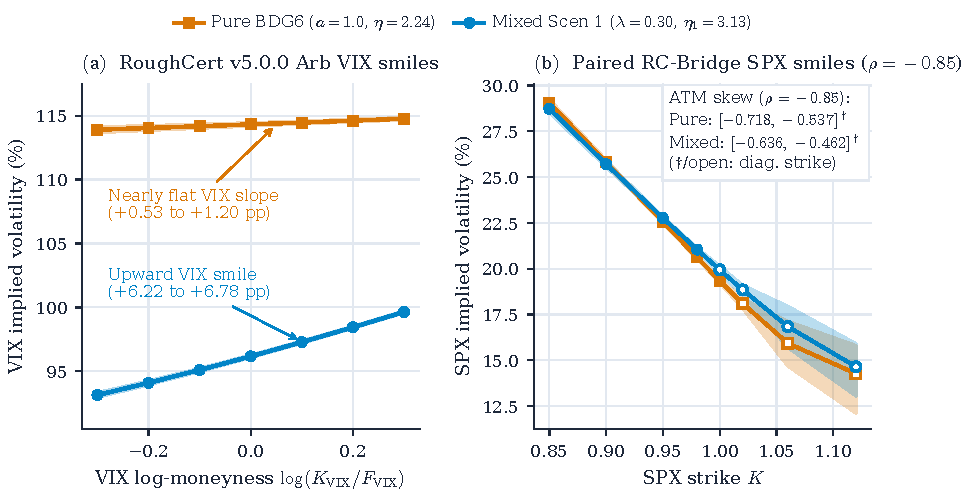
\includegraphics[width=\textwidth]{figures/fig_e6_joint_spx_vix.pdf}
  \caption{Joint SPX--VIX audit at $H=0.10$, $T=0.25$, $\xi_0=0.235^2$. (a) Arb-certified VIX smiles from \RoughCert{} \CompanionTag{} for Pure~BDG6 and Mixed~Scen.~1. (b) $65{,}536$-path \RCBridge{} SPX smiles at $\rho=-0.85$ (filled: asymptotic envelope; open: diagnostic).}
  \label{fig:e6_joint}
\end{figure}

Four conclusions follow, each with its epistemic status.
\begin{itemize}
  \item \emph{A certified VIX lift beside statistically controlled SPX skews.} At $\rho=-0.70$, where all three stencil strikes $\{e^{-0.02},1,e^{0.02}\}$ have asymptotic-envelope status for both models, Pure~BDG6 pairs a nearly flat Arb-certified VIX slope of $[\ESixPureVixSlopeLo,\ESixPureVixSlopeHi]\,\mathrm{pp}$ with an SPX ATM skew of $[\ESixPureSeventySkewLo,\ESixPureSeventySkewHi]$, whereas Mixed~Scen.~1 raises the VIX slope to $[\ESixMixVixSlopeLo,\ESixMixVixSlopeHi]\,\mathrm{pp}$ and keeps a steep SPX skew of $[\ESixMixSeventySkewLo,\ESixMixSeventySkewHi]$. The two certified VIX intervals are separated by at least $\ESixVixLiftLo\,\mathrm{pp}$, so the VIX lift is a property of the continuum models rather than a discretisation artefact; the SPX skews carry asymptotic-envelope guarantees with joint coverage at least $0.90$. At $\rho=-0.85$ (Figure~\ref{fig:e6_joint}(b)) the skews steepen to $[\ESixPureSkewLo,\ESixPureSkewHi]^\dagger$ (Pure~BDG6) and $[\ESixMixSkewLo,\ESixMixSkewHi]^\dagger$ (Mixed~Scen.~1), where the daggers mark diagnostic flags on the stencil.
  \item \emph{Refinement of the $\rho=-0.85$ stencils.} With one more level ($n_L=\RefFinestLevel$) and fresh seeds (Supplementary Table~S1), the Mixed~Scen.~1 stencil reaches asymptotic-envelope status and its skew interval narrows to $[\RefMixSkewLo,\RefMixSkewHi]$; only the call wing $K=1.06$ remains diagnostic. For Pure~BDG6 the skew interval becomes $[\RefPureSkewLo,\RefPureSkewHi]$, but the stencil stays flagged: at $K=1$ and $K=e^{0.02}$ the finest increment is resolved while the previous one is not (an emerging increment), and $K=1.06$ contracts too slowly.
  \item \emph{Coarse-grid skew estimates carry no bias control.} For Mixed~Scen.~1 at $\rho=-0.85$, a single-grid left-point simulation with $n=64$ gives an ATM skew point estimate of $\ESixMixCoarseSkew$. It falls inside the diagnostic bracket, but a single grid gives no estimate of its own discretisation bias, whereas \RCBridge{} reports the residual uncertainty together with the contraction warning.
  \item \emph{Stress test of the contraction gate.} Across the nine model--correlation rows ($\ESixStrikesTotal$ strike evaluations), \RCBridge{} reports no diagnostic strike for Pure~E14 at $\rho\in\{-0.85,-0.90\}$ and Pure~BDG6 at $\rho=-0.95$, and flags $\ESixTotalDiag$ strikes in total: $\ESixMixDiagHighRho$ of them in Mixed~Scen.~1 ($\eta_1=3.1305$) at $|\rho|\ge 0.85$ and $\ESixMixDiagAll$ in Mixed~Scen.~1 overall, where heavy variance tails slow the dyadic contraction. Theorem~\ref{thm:bridge_envelope}(iii) flags these strikes instead of certifying slow contraction, which tells a validator where finer grids or larger budgets are needed; the refinement above shows what one more level achieves for the two $\rho=-0.85$ rows.
\end{itemize}

\FloatBarrier
%
\section{Practical guidance, scope and conclusions}
\label{sec:conclusions}

This paper extended verified numerical certification from single-driver VIX derivatives \citep{AhmedEtAl2026RoughCert} to correlated SPX option pricing under rough volatility and treated full deterministic certification as a hypothesis. The theory predicts where that hypothesis must fail, the experiments locate the boundary, and the result is a workflow for volatility desks and model-validation teams.

\subsection{Operational guidance}

\begin{enumerate}[1.]
  \item \emph{Deterministic certification works without leverage and in mild regimes.} At $\rho=0$, Proposition~\ref{prop:twomoment} certifies ATM implied volatility to $25\bps$ up to $\eta T^H\in[\ETwoRhoZeroMin,\ETwoRhoZeroMax]$. At $\rho=-0.9$ the Put-Lipschitz bound of Theorem~\ref{thm:put_lipschitz} reaches $25\bps$ only for $\eta T^H\in[\ETwoRhoNineMin,\ETwoRhoNineMax]$, a contraction by a factor of $\ETwoCollapseMin$--$\ETwoCollapseMax$ that combines a leverage factor of $\ETwoLeverageMin$--$\ETwoLeverageMax$ with the loss of the second-order bound, as Theorem~\ref{thm:homotopy} predicts.
  \item \emph{Audit approximate kernels before simulating.} Theorem~\ref{thm:put_lipschitz} bounds the continuous-time kernel gap of Markovian and hybrid schemes in Arb before any path is drawn, and Lemma~\ref{lem:surrogate_mart} guarantees that the bound applies to every nonnegative kernel. With unclipped nodes, the certified \citet{BayerBreneis2023} $L^2$ and $L^1$ errors decay geometrically in $M$, and the certified hybrid IV gaps fall from $\EThreeBLPKapOneIV\bps$ ($\kappa=1$) to $\EThreeBLPKapEightIV\bps$ ($\kappa=8$). At calibrated vol-of-vol these first-order certificates are conservative (about $\EThreeMkTenMSixteenGapIV\bps$ against an empirical ATM error of at most $\EThreeMkTenMSixteenATMHi\bps$ for $M=16$), so they bound the kernel error but do not apportion the observed error.
  \item \emph{Keep conditional-Jensen smoothing out of the leverage integral.} Replacing $\sqrt{v_s}$ by $\E[\sqrt{v_s}\mid\G_i]$ inside $J_T$ removes a fraction $\Theta(n^{-2H})$ of the correlated quadratic variation and attenuates the effective correlation (Proposition~\ref{prop:jensen_pitfall}); in Experiments~E1, E4 and E5 the ablation is less accurate at every tested grid and has lower measured rates. Exact conditional expectation in the variance channel with an energy-conserving adapted $J_T$ (\RCCE{}) reduces the coarse-grid error by a factor of $\EOneRSSCeGainLow$ in E1 and shows rates comparable to the left-point scheme in E5.
  \item \emph{Separate sampling noise from continuum bias.} In calibrated regimes ($\eta\approx 1.9$, $\rho\approx -0.9$), \RCBridge{} gives \emph{asymptotic-envelope statistical(0.95)} enclosures across the smile from exact Schur-complement coarsening, pilot-fitted stopped-timer controls and unclamped contraction gates, and it flags strikes whose increments do not contract. Placed beside the Arb VIX brackets of \RoughCert{} \CompanionTag{}, these envelopes show that the VIX smile lift of the mixed model is a model property rather than a discretisation artefact.
\end{enumerate}

\subsection{Scope and limitations}

Six limits of the guarantees should be kept in view.
\begin{itemize}
  \item \emph{Deterministic and statistical guarantees differ.} Only \RCDet{} brackets and the kernel $L^2$, $L^1$ and price-gap bounds are \emph{Arb-certified}. \RCBridge{} intervals are \emph{asymptotic-envelope statistical(0.95)}, conditional on the tail hypothesis of Theorem~\ref{thm:bridge_envelope} and on approximately Gaussian shift means, or \emph{diagnostic}; ATM skews built from two strikes have joint coverage of at least $0.90$, and Arb inversion of a statistical interval does not change its status.
  \item \emph{Most envelopes rely on Case~(ii).} $\CaseTwoCount$ of the $\CaseTotalCount$ reference-envelope strikes use the assumed rate $\beta_{\mathrm{FSW}}$, which is valid for any true rate above $\beta_{\min}(H)$. Experiment~E5 supports this for $H\ge 0.10$ but not at $H=0.05$, and the very rough Regime~B ($H=0.07$) lies between the tested values.
  \item \emph{Finite grids.} The certifiability boundaries are the last certified points of finite bisections on a finite $(H,\eta T^H)$ grid, and all weak rates are fitted on grids up to $n=512$ (or $n=\RefFinestLevel$ in the refinement study). After refinement, $\RefFlagsVTwo$ strikes of the refined envelopes remain diagnostic.
  \item \emph{Martingale domain.} The software enforces $\rho\in[-1,0]$, which suffices for unit-forward parity. The positive-correlation strict-local-martingale result of \citet{Gassiat2019} requires nondegenerate volatility.
  \item \emph{Continuous time versus time stepping.} The Arb kernel-gap bounds concern $|C(K)-C_{\hat{K}}(K)|$ in continuous time; the time-discretisation bias $|C_{\hat{K}}(K)-C_{\hat{K},n}(K)|$ is audited separately by \RCBridge{}.
  \item \emph{Extensions.} Extending the two-field ledger and the exact-bridge envelope to affine rough Heston \citep{ElEuchRosenbaum2019,BayerBreneis2024}, to multi-factor path-dependent volatility \citep{AbiJaberIllandLi2025}, and to path-dependent equity exotics (cliquets, barriers), where Romano--Touzi conditioning no longer reduces to scalar Black--Scholes prices, remains open.
\end{itemize}

\FloatBarrier
%
\section*{CRediT authorship contribution statement}
\textbf{Eslam Ahmed:} Writing -- original draft, Visualization, Software, Methodology, Data curation, Conceptualization.
\textbf{Mohamed A. El-Beltagy:} Supervision, Conceptualization, Methodology, Validation, Data curation, Writing -- review \& editing.
\textbf{Ahmed Etman:} Writing -- review \& editing, Validation, Software, Formal analysis, Data curation.
\textbf{Sroor M. Elnady:} Writing -- review \& editing, Validation, Software, Formal analysis, Data curation.

\section*{Declaration of competing interest}
The authors declare that they have no known competing financial interests or personal relationships that could have appeared to influence the work reported in this paper.

\section*{Funding}
This work was supported by the Science, Technology \& Innovation Funding Authority (STDF), Egypt, under the Basic Sciences Grant, Project ID 50925. The funder had no role in the study design, analysis and interpretation, manuscript preparation or decision to submit the work for publication.

\section*{Data and code availability}
All benchmark inputs are synthetic model parameters taken from the cited publications; no market data are used. The Python implementation (Arb certification routines, exact-bridge RQMC envelopes and competitor implementations), the unit tests, the archived JSON results and the scripts that regenerate and check every table, figure and reported number are available in the \href{https://github.com/EslamAhmedGaber/RoughCert-SPX}{public repository} and its archived \href{\ReleaseURL}{release \ReleaseTag}. The VIX inputs of Experiment~E6 are taken from the companion working paper and software release \href{\CompanionURL}{\RoughCert{} \CompanionTag} \citep{AhmedEtAl2026RoughCert}. \ref{app:repro} describes the computational protocol.

\section*{Declaration of generative AI and AI-assisted technologies in the writing process}
The authors used ChatGPT and Claude to improve the readability of the manuscript. They reviewed and edited the text and take full responsibility for the published work.
%

{\small
\setlength{\bibsep}{3pt}
\bibliographystyle{elsarticle-num-names}
\bibliography{references}
}

\appendix
\section{Proofs of the main results}
\label{app:proofs}

\begin{proof}[Proof of Lemma~\ref{lem:surrogate_mart}]
$\hat{F}$ is a nonnegative local martingale, hence a supermartingale, so $\E[\hat{F}_T]\le1$. For $N\in\N$ let $\hat{I}_t=\int_0^t\hat{v}_s\dd s$ and $\tau_N=\inf\{t\in[0,T]:\hat{I}_t\ge N\}$, with $\inf\emptyset=T$. Since $\rho^2\hat{I}_{\tau_N}\le N$, Novikov's criterion gives $\E[\hat{F}_{\tau_N}]=1$, and $\mathbb{Q}_N\coloneqq\hat{F}_{\tau_N}\cdot\mathbb{Q}$ is a probability measure equivalent to $\mathbb{Q}$. By Girsanov's theorem, $\tilde{W}_t=W_t^{(1)}-\rho\int_0^{t\wedge\tau_N}\hat{\sigma}_s\dd s$ is a $\mathbb{Q}_N$-Brownian motion, and
\[
  \begin{aligned}
  \hat{Y}_s&=\int_0^s\hat{K}(s-u)\dd\tilde{W}_u+\rho\int_0^{s\wedge\tau_N}\hat{K}(s-u)\,\hat{\sigma}_u\dd u \TCrel \le\tilde{Y}_s\coloneqq\int_0^s\hat{K}(s-u)\dd\tilde{W}_u,
  \end{aligned}
\]
because $\rho\le0$, $\hat{K}\ge0$ and $\hat{\sigma}\ge0$. As each $\Phi_s$ is nondecreasing, $\hat{I}_T\le\tilde{I}_T\coloneqq\int_0^T\Phi_s(\tilde{Y}_s)\dd s$, and $\tilde{I}_T$ has under $\mathbb{Q}_N$ the law that $\hat{I}_T$ has under $\mathbb{Q}$. On $\{\hat{I}_T<N\}$ we have $\tau_N=T$ and $\hat{F}_T=\hat{F}_{\tau_N}$, hence
\[
  \begin{aligned}
  \E[\hat{F}_T]&\ge\E\bigl[\hat{F}_{\tau_N}\mathbf{1}_{\{\tau_N=T\}}\bigr]=\mathbb{Q}_N(\tau_N=T) \TCrel \ge\mathbb{Q}_N(\hat{I}_T<N)\ge1-\mathbb{Q}_N(\tilde{I}_T\ge N) \TCrel =1-\mathbb{Q}(\hat{I}_T\ge N).
  \end{aligned}
\]
The right-hand side tends to $1$ as $N\to\infty$ because $\E[\hat{I}_T]<\infty$, so $\E[\hat{F}_T]=1$. For rough and mixed rough Bergomi, $\Phi_s(y)=\xi_0(s)[\lambda\exp(\eta_1y-\tfrac12\eta_1^2a_s)+(1-\lambda)\exp(\eta_2y-\tfrac12\eta_2^2a_s)]$ with $a_s=\int_0^s\hat{K}(u)^2\dd u$ is nondecreasing because $\eta_1,\eta_2\ge0$; Markovian kernels with $w_j\ge0$ and hybrid kernels are nonnegative.
\end{proof}

\begin{proof}[Proof of Theorem~\ref{thm:ledger}]
(i) Since $\sqrt{v_s}-\hat{\sigma}_s$ is adapted and lies in $L^2([0,T]\times\Omega)$, the It\^o isometry gives
\[
  \begin{aligned}
  \E\!\left[(J_T-\hat{J}_T)^2\right]
  &= \E\!\left[\left(\int_0^T(\sqrt{v_s}-\hat{\sigma}_s)\dd W_s^{(1)}\right)^2\right]
  \TCrel = \E\!\left[\int_0^T(\sqrt{v_s}-\hat{\sigma}_s)^2\dd s\right]
  = E_J^2.
  \end{aligned}
\]
(ii) Pathwise, the reverse triangle inequality in $L^2(0,T)$ gives
\[
  \begin{aligned}
  \bigl|\sqrt{I_T}-\sqrt{\hat{I}_T}\bigr|
  &= \bigl|\norm{\sqrt{v}}_{L^2(0,T)}-\norm{\hat{\sigma}}_{L^2(0,T)}\bigr|
  \TCrel \le \norm{\sqrt{v}-\hat{\sigma}}_{L^2(0,T)}.
  \end{aligned}
\]
Squaring and taking expectations gives the first bound in \eqref{eq:minkowski_coupling}. For the second, write $|I_T-\hat{I}_T|$ as the product of $|\sqrt{I_T}-\sqrt{\hat{I}_T}|$ and $\sqrt{I_T}+\sqrt{\hat{I}_T}$ and apply the Cauchy--Schwarz and Minkowski inequalities:
\[
  \begin{aligned}
  E_I
  &\le \norm{\sqrt{I_T}-\sqrt{\hat{I}_T}}_{L^2(\mathbb{Q})} \TCbr \norm{\sqrt{I_T}+\sqrt{\hat{I}_T}}_{L^2(\mathbb{Q})}
  \TCrel \le E_J\left(\sqrt{\E[I_T]}+\sqrt{\E[\hat{I}_T]}\right).
  \end{aligned}
\]
(iii) Let $a_s=\Var(Y_s)$, $\hat{a}_s=\Var(\hat{Y}_s)$ and $c_s=\Cov(Y_s,\hat{Y}_s)$, so that $\Var(Y_s-\hat{Y}_s)=a_s+\hat{a}_s-2c_s$. Since
\[
  \begin{gathered}
  \sqrt{v_s}=\sqrt{\xi_0(s)}\exp\!\left(\tfrac12\eta Y_s-\tfrac14\eta^2 a_s\right),
  \TCsep
  \hat{\sigma}_s=\sqrt{\xi_0(s)}\exp\!\left(\tfrac12\eta\hat{Y}_s-\tfrac14\eta^2\hat{a}_s\right),
  \end{gathered}
\]
we have $\E[v_s]=\E[\hat{v}_s]=\xi_0(s)$ and, by the Gaussian moment-generating function of $\tfrac12\eta(Y_s+\hat{Y}_s)$,
\[
  \begin{aligned}
  \E\!\left[\sqrt{v_s}\,\hat{\sigma}_s\right]
  &= \xi_0(s)\exp\Bigl(-\tfrac14\eta^2(a_s+\hat{a}_s) \TCbr + \tfrac18\eta^2(a_s+\hat{a}_s+2c_s)\Bigr)
  \TCrel = \xi_0(s)\exp\!\left(-\tfrac{\eta^2}{8}\Var(Y_s-\hat{Y}_s)\right).
  \end{aligned}
\]
Hence $\E[(\sqrt{v_s}-\hat{\sigma}_s)^2]=2\xi_0(s)[1-\exp(-\tfrac{\eta^2}{8}\Var(Y_s-\hat{Y}_s))]$, and Tonelli's theorem gives \eqref{eq:mehler_ej}. For $\hat{Y}_s=\int_0^s\hat{K}(s-u)\dd W_u^{(1)}$, the It\^o isometry gives $\Var(Y_s-\hat{Y}_s)=\int_0^s(K_H(u)-\hat{K}(u))^2\dd u$.
\end{proof}

\begin{proof}[Proof of Theorem~\ref{thm:put_lipschitz}]
By Lemma~\ref{lem:surrogate_mart} with $\hat{K}=K_H$ and by the hypothesis $\E[\hat{F}_T]=1$, both $S_T$ and the surrogate spot $\hat{S}_T$ are true martingales with mean $1$, so Put--Call parity gives $C(K)-\hat{C}(K)=P(K)-\hat{P}(K)$ for every $K>0$. Write $P_\BS(e^u,K,\Sigma^2)=K\Phi(-d_-)-e^u\Phi(-d_+)$ for $u\in\R$ and $\Sigma>0$, with $d_\pm=(u-\log K)/\Sigma\pm\Sigma/2$. Using $e^u\phi(d_+)=K\phi(d_-)$,
\[
  \begin{gathered}
  -\frac{\partial P_\BS}{\partial u} = e^u\Phi(-d_+) \ge 0,
  \TCsep
  \frac{\partial P_\BS}{\partial \Sigma} = K\phi(d_-) \in \left(0,\frac{K}{\sqrt{2\pi}}\right].
  \end{gathered}
\]
Since $P_\BS\ge0$, $0\le e^u\Phi(-d_+)\le K\Phi(-d_-)\le K$ for all $(u,\Sigma)\in\R\times(0,\infty)$, and $P_\BS(e^u,K,0)=(K-e^u)_+$ is $K$-Lipschitz in $u$ as well. With $u=\rho J_T-\tfrac12\rho^2 I_T$, $\Sigma=\bar{\rho}\sqrt{I_T}$ and the surrogate counterparts $\hat{u}$, $\hat{\Sigma}$, the mean value theorem gives
\[
  \begin{aligned}
  &\bigl|P_\BS(F_T,K,\bar{\rho}^2 I_T)-P_\BS(\hat{F}_T,K,\bar{\rho}^2\hat{I}_T)\bigr|
  \TCrel \le K|\rho|\,|J_T-\hat{J}_T| + \frac{K\rho^2}{2}|I_T-\hat{I}_T| \TCbr + \frac{K\bar{\rho}}{\sqrt{2\pi}}\bigl|\sqrt{I_T}-\sqrt{\hat{I}_T}\bigr|.
  \end{aligned}
\]
Taking expectations, bounding $\E|X|\le\norm{X}_{L^2(\mathbb{Q})}$ and using Theorem~\ref{thm:ledger}(i)--(ii) gives \eqref{eq:put_lipschitz}. The splitting \eqref{eq:three_way} is the triangle inequality.
\end{proof}

\begin{proof}[Proof of Theorem~\ref{thm:homotopy}]
\emph{Identity.} Since $I_\theta>0$ a.s.\ and $\bar{\rho}>0$, the function $g(\theta)=C_\BS(F_\theta,K,\bar{\rho}^2 I_\theta)$ is continuously differentiable on $[0,1]$ with
\[
  \begin{aligned}
  g'(\theta) &= \Delta_\BS(\theta)F_\theta\bigl(\rho(J_T-\hat{J}_T)-\tfrac12\rho^2(I_T-\hat{I}_T)\bigr)
               \TCbr + \bar{\rho}^2\mathcal{V}_\BS(\theta)(I_T-\hat{I}_T).
  \end{aligned}
\]
By Put--Call parity, $\mathcal{V}_\BS(\theta)=\partial_V P_\BS(F_\theta,K,\bar{\rho}^2 I_\theta)=K\phi(d_-)/(2\bar{\rho}\sqrt{I_\theta})\le K/(2\bar{\rho}\sqrt{2\pi I_\theta})$, and since $I_\theta$ is affine in $\theta$, $\int_0^1 |I_T-\hat{I}_T|\,I_\theta^{-1/2}\dd\theta = 2|\sqrt{I_T}-\sqrt{\hat{I}_T}|\in L^2(\mathbb{Q})$. The Put-delta bound $0\le(1-\Delta_\BS(\theta))F_\theta\le K$ and \eqref{eq:homotopy_integrability} dominate the remaining terms, so Fubini's theorem applies to $\E[g(1)-g(0)]=\E\int_0^1g'(\theta)\dd\theta$ and yields \eqref{eq:homotopy}; no negative moment of $I_\theta$ is needed.

\emph{Integrability for deterministic surrogates.} Let $\hat{\sigma}$ be deterministic with $\hat{I}\coloneqq\hat{I}_T\in(0,\infty)$. Then $\hat{J}_T\sim\mathcal{N}(0,\hat{I})$ and $\hat{F}_T$ is lognormal with finite moments of all orders. Convexity of the exponential gives $F_\theta\le(1-\theta)\hat{F}_T+\theta F_T$, so it suffices to bound $\E[\hat{F}_TX]$ and $\E[F_TX]$ for $X\in\{|J_T|,|\hat{J}_T|,I_T,\hat{I}\}$. By Cauchy--Schwarz, $\E[\hat{F}_TX]\le(\E\hat{F}_T^2)^{1/2}(\E X^2)^{1/2}<\infty$, because $\E[J_T^2]=\E[I_T]=I_0$, $\E[\hat{J}_T^2]=\hat{I}$ and $\E[I_T^2]\le I_0^2e^{\eta^2T^{2H}}$. For the terms with $F_T$, Lemma~\ref{lem:surrogate_mart} gives $\E[F_T]=1$; under $\mathbb{Q}^F\coloneqq F_T\cdot\mathbb{Q}$ the process $W_t^F=W_t^{(1)}-\rho\int_0^t\sqrt{v_s}\dd s$ is a Brownian motion, and, as in the proof of the lemma, $Y_s\le Y_s^F\coloneqq\int_0^sK_H(s-u)\dd W_u^F$, so $v_s\le\xi_0(s)\cE(\eta Y_s^F)$ and $\E^F[I_T]\le I_0$. Hence $\E[F_TI_T]\le I_0$, $\E[F_T\hat{I}]=\hat{I}$,
\[
  \begin{gathered}
  \E[F_T|J_T|]=\E^F\Bigl|\int_0^T\!\sqrt{v_s}\dd W_s^F+\rho I_T\Bigr|\le I_0^{1/2}+|\rho|I_0,
  \TCsep
  \E[F_T|\hat{J}_T|]\le\hat{I}^{1/2}+|\rho|\,\hat{I}^{1/2}I_0^{1/2},
  \end{gathered}
\]
where the last bound uses $|\int_0^T\hat{\sigma}_s\sqrt{v_s}\dd s|\le(\hat{I}I_T)^{1/2}$. Thus \eqref{eq:homotopy_integrability} holds. If moreover $\hat{I}=I_0$, then $\hat{J}_T\sim\mathcal{N}(0,I_0)$ and the Gaussian semigroup gives $\hat{C}(K)=\E[C_\BS(\hat{F}_T,K,\bar{\rho}^2I_0)]=C_\BS(1,K,I_0)$ for every such surrogate.

\emph{Part (a).} For $\rho=0$, $F_T=\hat{F}_T=1$ and $C(K)-\hat{C}(K)=\E[h(I_T)]-h(I_0)$ with $h(V)=C_\BS(1,K,V)$ and $\E[I_T]=I_0$. For $K\ne1$, the first two derivatives of $h$ vanish faster than any power of $V$ as $V\downarrow0$ and $h''(V)\to0$ as $V\to\infty$, so $\sup_{V>0}|h''(V)|<\infty$, and Taylor's theorem with Lagrange remainder gives the stated bound. For $K=1$, Proposition~\ref{prop:twomoment} with $m=I_0$ and $v=\Var(I_T)$ gives $0\le\varphi_1(m)-\E[\varphi_1(I_T)]\le\varphi_1(m)-L(v)$, and $L$ is differentiable at $v=0$ with $L(0)=\varphi_1(m)$. For flat $\xi_0$, $R_H(s,u)\le T^{2H}$ gives $\Var(I_T)=\xi_0^2\int\!\!\int(e^{\eta^2R_H}-1)\le I_0^2(e^{\eta^2T^{2H}}-1)$.

\emph{Part (b).} Take $\hat{\sigma}_s=\sqrt{\xi_0(s)}$, which has $\hat{I}_T=I_0$. Expanding formally as $\eta\to 0$, $\sqrt{v_s}-\hat{\sigma}_s=\tfrac12\eta\sqrt{\xi_0(s)}Y_s + O(\eta^2)$ and $I_T-I_0=\eta\int_0^T\xi_0(s)Y_s\dd s + O(\eta^2)$, while at $\eta=0$, $F_\theta\equiv F_0=\exp(\rho\int_0^T\sqrt{\xi_0(r)}\dd W_r^{(1)}-\tfrac12\rho^2 I_0)$ and $I_\theta\equiv I_0$. Since $\sqrt{\xi_0(s)}Y_s$ is adapted, Malliavin integration by parts \citep{Nualart2006} with $D_s F_0=\rho\sqrt{\xi_0(s)}F_0$ gives
\[
  \begin{aligned}
  &\E\!\left[\rho\Delta_\BS(0)F_0\int_0^T\tfrac12\eta\sqrt{\xi_0(s)}Y_s\dd W_s^{(1)}\right]
  \TCrel = \tfrac12\rho^2\eta\int_0^T \xi_0(s)\,\E\!\left[F_0(\Delta_\BS(0)+F_0\Gamma_\BS(0))\,Y_s\right]\dd s.
  \end{aligned}
\]
The $O(\eta)$ part of the second term of \eqref{eq:homotopy} is
\[
  \eta\int_0^T\xi_0(s)\,\E\bigl[(\bar{\rho}^2\mathcal{V}_\BS(0)-\tfrac12\rho^2\Delta_\BS(0)F_0)\,Y_s\bigr]\dd s;
\]
adding it cancels the terms in $\tfrac12\rho^2\Delta_\BS(0)F_0$, and the Gamma--Vega identity $\mathcal{V}_\BS=\tfrac12 F^2\Gamma_\BS$ reduces the sum to
\[
  \tfrac12\eta\int_0^T\xi_0(s)\,\E\bigl[F_0^2\Gamma_\BS(F_0,K,\bar{\rho}^2 I_0)\,Y_s\bigr]\dd s.
\]
The pair $(\log F_0,Y_s)$ is jointly Gaussian with
\[
  \Cov(\log F_0,Y_s)=\rho\int_0^s\sqrt{\xi_0(u)}\,K_H(s-u)\dd u,
\]
so Stein's lemma and the identity $\E[C_\BS(e^x F_0,K,\bar{\rho}^2 I_0)]=C_\BS(e^x,K,I_0)$ give
\[
  \begin{aligned}
    &\E\!\left[F_0^2\Gamma_\BS(F_0,K,\bar{\rho}^2 I_0)\,Y_s\right]
    \TCrel = \Cov(\log F_0,Y_s)\left.\frac{\partial}{\partial x}\!\left(e^{2x}\Gamma_\BS(e^x,K,I_0)\right)\right|_{x=0} \\
    &\qquad = \Cov(\log F_0,Y_s)\,\frac{2\mathcal{V}_\BS(1,K,I_0)}{I_0}\left(\log K + \frac{I_0}{2}\right),
  \end{aligned}
\]
using $e^{2x}\Gamma_\BS(e^x,K,I_0)=e^x\phi(d_+)/\sqrt{I_0}$ and $1-d_+/\sqrt{I_0}=(\log K)/I_0+\tfrac12$ at $x=0$. Integrating over $s$ gives \eqref{eq:homotopy_leverage}. For flat $\xi_0$, $C^{x\xi}/I_0 = \rho\eta\sqrt{\xi_0}\,\sqrt{2H}\,T^{H+1/2}/((H+\tfrac12)(H+\tfrac32))$. This calculation identifies the formal coefficient. It supplies no remainder estimate.
\end{proof}

\begin{proof}[Proof of Proposition~\ref{prop:twomoment}]
Write $u=\tfrac12\sqrt{V}>0$, so $\varphi_1(V)=2\Phi(u)-1$ and $\dd u/\dd V=1/(8u)$. Using $\phi'(u)=-u\phi(u)$, three differentiations give
\[
  \begin{gathered}
  \varphi_1'(V) = \frac{\phi(u)}{4u} > 0,
  \TCsepq
  \varphi_1''(V) = -\frac{u^{-3}+u^{-1}}{32}\,\phi(u) < 0,
  \TCsepq
  \varphi_1'''(V) = \frac{3u^{-5}+2u^{-3}+u^{-1}}{256}\,\phi(u) > 0.
  \end{gathered}
\]
Concavity gives $\E[\varphi_1(I_T)]\le\varphi_1(m)$. For the lower bound, let $x_*=m+v/m>0$ and let $q$ be the quadratic with $q(0)=0$, $q(x_*)=\varphi_1(x_*)$ and $q'(x_*)=\varphi_1'(x_*)$:
\[
  q(x) = \frac{\varphi_1(x_*)}{x_*}\,x + \left(\varphi_1'(x_*)-\frac{\varphi_1(x_*)}{x_*}\right)\frac{x(x-x_*)}{x_*}.
\]
Let $h=\varphi_1-q$ on $[0,\infty)$. Then $h(0)=h(x_*)=h'(x_*)=0$ and $h'''=\varphi_1'''>0$, so $h''$ is strictly increasing. By Rolle's theorem there are $c_1\in(0,x_*)$ with $h'(c_1)=0$ and $c_2\in(c_1,x_*)$ with $h''(c_2)=0$. Hence $h''<0$ on $(0,c_2)$ and $h''>0$ on $(c_2,\infty)$, so $h'$ decreases on $(0,c_2)$ and increases on $(c_2,\infty)$; therefore $h'>0$ on $(0,c_1)$, $h'<0$ on $(c_1,x_*)$ and $h'>0$ on $(x_*,\infty)$, and $h\ge 0$ on $[0,\infty)$. Since $\E[I_T(I_T-x_*)]=(m^2+v)-(m+v/m)m=0$,
\[
  \begin{aligned}
  \E[\varphi_1(I_T)] &\ge \E[q(I_T)] = \frac{m}{x_*}\varphi_1(x_*) \TCrel = \frac{m^2}{m^2+v}\,\varphi_1\!\left(m+\frac{v}{m}\right),
  \end{aligned}
\]
with equality for the two-point law on $\{0,x_*\}$. Finally, $\varphi_1(0)=0$ and $\varphi_1''<0$ give $\frac{\dd}{\dd x}(\varphi_1(x)/x)=(x\varphi_1'(x)-\varphi_1(x))/x^2<0$, so $L(v)=m\,\varphi_1(x_*)/x_*$ is strictly decreasing in $v$.
\end{proof}

\begin{proof}[Proof of Proposition~\ref{prop:jensen_pitfall}]
(i) For $s\in[t_i,t_{i+1}]$ let $\mu_s=\E[Y_s\mid\G_i]$, $D_i(s)=\Var(Y_s\mid\G_i)$ (deterministic, as the conditioning is Gaussian) and $g_s=\E[\sqrt{v_s}\mid\G_i]$. Since $Y_s\mid\G_i\sim\mathcal{N}(\mu_s,D_i(s))$, $g_s=\sqrt{\xi_0}\exp(\tfrac12\eta\mu_s-\tfrac14\eta^2s^{2H}+\tfrac18\eta^2D_i(s))$ and $\Var(\sqrt{v_s}\mid\G_i)=\E[v_s\mid\G_i](1-e^{-\eta^2D_i(s)/4})$. With $\sigma_i^{\mathrm{Jen}}=\Delta t^{-1}\int_{t_i}^{t_{i+1}}g_s\dd s$,
\[
  \begin{aligned}
  &\E[I_T-I_{\mathrm{ad}}]
  =\xi_0\sum_{i=0}^{n-1}\int_{t_i}^{t_{i+1}}\Bigl(1-e^{-\eta^2D_i(s)/4}\Bigr)\dd s
  \TCbr +\sum_{i=0}^{n-1}\E\int_{t_i}^{t_{i+1}}\bigl(g_s-\sigma_i^{\mathrm{Jen}}\bigr)^2\dd s,
  \end{aligned}
\]
where the second sum is the nonnegative time-Jensen term. Because $\G_i\subset\F_{t_i}^{W^{(1)}}$, $D_i(s)\ge\Var(Y_s\mid\F_{t_i}^{W^{(1)}})=\int_{t_i}^sK_H(s-u)^2\dd u=(s-t_i)^{2H}$; dropping the second sum gives the lower bound in \eqref{eq:jensen_deficit}, and expanding $1-e^{-x}=x+O(x^2)$ gives its asymptotic form. For the upper bound, $Y_{t_i}$ is $\G_i$-measurable, so $D_i(s)\le\Var(Y_s-Y_{t_i})\le c_H\Delta t^{2H}$, where $c_H=1+2H\int_0^\infty((1+x)^{H-1/2}-x^{H-1/2})^2\dd x<\infty$; this bounds the first sum by $\tfrac14\xi_0\eta^2Tc_H\Delta t^{2H}$. For the time-Jensen term, $\E[(\mu_s-\mu_{s'})^2]\le\Var(Y_s-Y_{s'})\le c_H|s-s'|^{2H}$, $|s^{2H}-s'^{2H}|\le|s-s'|^{2H}$ and $|D_i(s)-D_i(s')|\le c'|s-s'|^{H}$ with $c'=T^H(1+2c_H^{1/2})$; with the uniformly bounded lognormal moments of $g_s$ these give $\E[(g_s-g_{s'})^2]\le c\,\Delta t^{2H}$ on each cell, so the time-Jensen term is at most $cT\Delta t^{2H}$. Hence $\delta_n=\Theta(\Delta t^{2H})=\Theta(n^{-2H})$.

(ii) $\E[I_{\mathrm{CE}}]=\E[\E[I_T\mid\G_n]]=\E[I_T]$, so $\rho_{\mathrm{eff}}^2=\rho^2\E[I_{\mathrm{ad}}]/\E[I_T]=\rho^2(1-\delta_n)$, and $|\rho_{\mathrm{eff}}|=|\rho|\sqrt{1-\delta_n}=|\rho|(1-\Theta(n^{-2H}))$ by (i).
\end{proof}

\begin{lemma}[Exact unbiasedness of the discrete stopped-timer control]
\label{lem:stopped_cv}
For any uniform grid $n\ge 1$, $\rho\in[-1,0]$, deterministic $Q_{\mathrm{var}}>0$ and $(\F_{t_i}^{W^{(1)}})$-adapted $\sigma_i\ge 0$, let $A_{i+1}=\rho^2\Delta t\sum_{j=0}^{i}\sigma_j^2$ and $\alpha_i=\mathbf{1}_{\{A_{i+1}\le Q_{\mathrm{var}}\}}$ for $i=0,\dots,n-1$. Let $I_\tau=\Delta t\sum_{i=0}^{n-1}\alpha_i\sigma_i^2$ and $F_\tau=\exp(\rho\sum_{i=0}^{n-1}\alpha_i\sigma_i\Delta W_i^{(1)}-\tfrac12\rho^2 I_\tau)$. Then $\rho^2 I_\tau\le Q_{\mathrm{var}}$ a.s.\ and
\[
  \begin{gathered}
  \E\!\left[C_\BS\!\left(F_\tau,\,K,\,Q_{\mathrm{var}}-\rho^2 I_\tau\right)\right]
  = C_\BS(1,K,Q_{\mathrm{var}})
  \TCsep\text{for every }K>0.
  \end{gathered}
\]
\end{lemma}

\begin{proof}
The cumulative sum $A_{i+1}$ is nondecreasing in $i$ and $\F_{t_i}^{W^{(1)}}$-measurable, so $\alpha_i$ is $\F_{t_i}^{W^{(1)}}$-measurable, nonincreasing in $i$ and independent of $\Delta W_i^{(1)}$. Let $I_k=\Delta t\sum_{i=0}^{k-1}\alpha_i\sigma_i^2$, $F_k=\exp(\rho\sum_{i=0}^{k-1}\alpha_i\sigma_i\Delta W_i^{(1)}-\tfrac12\rho^2 I_k)$ and $M_k=C_\BS(F_k,K,Q_{\mathrm{var}}-\rho^2 I_k)$ for $k=0,\dots,n$. Since $\alpha$ is nonincreasing, $\rho^2I_k\le Q_{\mathrm{var}}$ a.s.\ for every $k$. Let $\Delta q_{k-1}=\rho^2\Delta t\,\alpha_{k-1}\sigma_{k-1}^2$, so that $\Delta q_{k-1}\le Q_{\mathrm{var}}-\rho^2 I_{k-1}$ and
\[
  \begin{gathered}
  F_k=F_{k-1}\exp\!\left(\sqrt{\Delta q_{k-1}}\,Z-\tfrac12\Delta q_{k-1}\right),\TCsep Z=-\Delta W_{k-1}^{(1)}/\sqrt{\Delta t},
  \end{gathered}
\]
where $Z\sim\mathcal{N}(0,1)$ is independent of $\F_{t_{k-1}}^{W^{(1)}}$. For $F>0$ and $0\le\Delta q\le V$, the Gaussian semigroup identity
\[
  \E\bigl[C_\BS\bigl(F e^{\sqrt{\Delta q}\,Z-\Delta q/2},K,V-\Delta q\bigr)\bigr]=C_\BS(F,K,V)
\]
gives $\E[M_k\mid\F_{t_{k-1}}^{W^{(1)}}]=M_{k-1}$, and backward induction gives $\E[M_n]=M_0=C_\BS(1,K,Q_{\mathrm{var}})$.
\end{proof}

\begin{proof}[Proof of Theorem~\ref{thm:bridge_envelope}]
The control weights $(W_\ell,W_{\Delta,\ell})$ are fitted on independent pilot shifts and held fixed, and every control has zero mean by Lemma~\ref{lem:stopped_cv}, $\E[F_T^{(n_\ell)}]=1$, $\E[I_{\mathrm{left}}^{(n_\ell)}]=\Delta t\sum_i\xi_0(t_i)$ and $\E[J_{\mathrm{left}}^{(n_\ell)}]=0$. Conditional on the pilot, the $R$ shift means of $C_L$ and of $\Delta_L$ are independent, identically distributed and unbiased for $C^{(n_L)}(K)$ and $\Delta_L(K)$. The Student-$t_{R-1}$ statements below are exact if these means are Gaussian and are asymptotic under a studentized central limit theorem (for example, increasing independent shifts with fixed paths per shift and finite positive variance). The events $\mathcal{A}_1=\{|\bar{C}_L - C^{(n_L)}| \le t\,s_L\}$ and $\mathcal{A}_2=\{|\Delta_L| \le d_L^{\mathrm{hi}}\}$ each have probability at least $1-\alpha/2$, so $\mathbb{P}(\mathcal{A}_1\cap\mathcal{A}_2)\ge 1-\alpha$. On $\mathcal{A}_1\cap\mathcal{A}_2$ and the stated tail event, since $d_{\mathrm{eff}}^{\mathrm{hi}}\ge d_L^{\mathrm{hi}}$ and $x\mapsto1/(2^x-1)$ is decreasing, the tail hypothesis with $\beta\ge\beta_{\mathrm{used}}$ gives
\[
  |C(K)-C^{(n_L)}(K)|\le\frac{\gamma_{\mathrm{sf}}|\Delta_L|}{2^\beta-1}\le\frac{\gamma_{\mathrm{sf}}\,d_{\mathrm{eff}}^{\mathrm{hi}}}{2^{\beta_{\mathrm{used}}}-1}=B_L(K),
\]
so $|C(K)-\bar{C}_L(K)|\le t\,s_L + B_L(K)$, and clipping to the no-arbitrage bounds $[(1-K)_+,1]$ preserves coverage. In Case~(i), the expansion hypothesis with $c_K\ne0$ makes $\hat{\beta}_{\mathrm{emp}}$ consistent for $\beta$ as $n_L\to\infty$ and relative increment errors vanish on the asymptotically fine levels used in the fit; since $\beta_{\mathrm{used}}\le0.85\hat{\beta}_{\mathrm{emp}}$, $\mathbb{P}(\beta_{\mathrm{used}}\le\beta)\to1$. In Case~(ii), $\beta_{\mathrm{used}}=\beta_{\mathrm{FSW}}$; under geometric increments, $\beta\ge\beta_{\min}(H)$ is equivalent to $1/(2^\beta-1)\le\gamma_{\mathrm{sf}}/(2^{\beta_{\mathrm{FSW}}}-1)$, and the geometric tail without the safety factor is bounded by the reported budget. Black--Scholes prices are strictly increasing in volatility, so outward-rounded Arb inversion of $[C_{\mathrm{lo}},C_{\mathrm{hi}}]$ encloses $\IV(K)$ whenever $C(K)\in[C_{\mathrm{lo}},C_{\mathrm{hi}}]$. The interval \eqref{eq:skew_interval} contains the finite-difference skew whenever both stencil strikes are covered, which by the Bonferroni inequality has probability at least $1-2\alpha$.
\end{proof}
%
\section{Computational protocol and traceability}
\label{app:repro}

\paragraph{Environment and timing.}
Each run used a single thread. E1--E6 used Python 3.12.4, NumPy 2.2.6, SciPy 1.14.1, python-flint 0.9.0 and mpmath 1.3.0. The refinement and decomposition studies used Python 3.12.14, NumPy 2.5.3, SciPy 1.18.1, python-flint 0.8.0, mpmath 1.4.1 and SymPy 1.14.0. In both environments, 52 decimal digits give \ArbBits{} Arb bits. Cold setup includes factorisation, node fitting or hybrid covariance assembly. Solve time includes path generation, payoff evaluation, controls and implied-volatility inversion.

\paragraph{Rounding and randomisation.}
Certified endpoints round outwards. A call upper bound of one gives an infinite upper implied volatility. Arb model inputs use their stated decimal values. Scrambled Sobol points use SciPy's linear matrix scramble and digital shift, antithetic pairing and archived seeds. Two pilot shifts fit the controls independently of the main shifts. E4 competitors share random numbers within regimes. Some E6 shifts overlap within model families. Refinement seeds start at $20262000$ and are disjoint from the reference seeds.

\paragraph{Traceability.}
The \href{\ReleaseURL}{version \ReleaseTag{} archive} includes the inputs and results. The table generator records the raw value, rounding rule and printed value for each numerical macro. It rounds lower endpoints and lower bounds on improvement factors downwards, and upper endpoints and error bounds upwards. Point estimates use nearest rounding. Supplementary Table~S6 identifies the scripts that generate the tables and figures. The independent programs behind Supplementary Table~S5 use separate implementations.
%
\end{document}
